\documentclass[twoside]{book}

% Packages required by doxygen
\usepackage{fixltx2e}
\usepackage{calc}
\usepackage{doxygen}
\usepackage[export]{adjustbox} % also loads graphicx
\usepackage{graphicx}
\usepackage[utf8]{inputenc}
\usepackage{makeidx}
\usepackage{multicol}
\usepackage{multirow}
\PassOptionsToPackage{warn}{textcomp}
\usepackage{textcomp}
\usepackage[nointegrals]{wasysym}
\usepackage[table]{xcolor}

% Font selection
\usepackage[T1]{fontenc}
\usepackage[scaled=.90]{helvet}
\usepackage{courier}
\usepackage{amssymb}
\usepackage{sectsty}
\renewcommand{\familydefault}{\sfdefault}
\allsectionsfont{%
  \fontseries{bc}\selectfont%
  \color{darkgray}%
}
\renewcommand{\DoxyLabelFont}{%
  \fontseries{bc}\selectfont%
  \color{darkgray}%
}
\newcommand{\+}{\discretionary{\mbox{\scriptsize$\hookleftarrow$}}{}{}}

% Page & text layout
\usepackage{geometry}
\geometry{%
  a4paper,%
  top=2.5cm,%
  bottom=2.5cm,%
  left=2.5cm,%
  right=2.5cm%
}
\tolerance=750
\hfuzz=15pt
\hbadness=750
\setlength{\emergencystretch}{15pt}
\setlength{\parindent}{0cm}
\setlength{\parskip}{3ex plus 2ex minus 2ex}
\makeatletter
\renewcommand{\paragraph}{%
  \@startsection{paragraph}{4}{0ex}{-1.0ex}{1.0ex}{%
    \normalfont\normalsize\bfseries\SS@parafont%
  }%
}
\renewcommand{\subparagraph}{%
  \@startsection{subparagraph}{5}{0ex}{-1.0ex}{1.0ex}{%
    \normalfont\normalsize\bfseries\SS@subparafont%
  }%
}
\makeatother

% Headers & footers
\usepackage{fancyhdr}
\pagestyle{fancyplain}
\fancyhead[LE]{\fancyplain{}{\bfseries\thepage}}
\fancyhead[CE]{\fancyplain{}{}}
\fancyhead[RE]{\fancyplain{}{\bfseries\leftmark}}
\fancyhead[LO]{\fancyplain{}{\bfseries\rightmark}}
\fancyhead[CO]{\fancyplain{}{}}
\fancyhead[RO]{\fancyplain{}{\bfseries\thepage}}
\fancyfoot[LE]{\fancyplain{}{}}
\fancyfoot[CE]{\fancyplain{}{}}
\fancyfoot[RE]{\fancyplain{}{\bfseries\scriptsize Generated by Doxygen }}
\fancyfoot[LO]{\fancyplain{}{\bfseries\scriptsize Generated by Doxygen }}
\fancyfoot[CO]{\fancyplain{}{}}
\fancyfoot[RO]{\fancyplain{}{}}
\renewcommand{\footrulewidth}{0.4pt}
\renewcommand{\chaptermark}[1]{%
  \markboth{#1}{}%
}
\renewcommand{\sectionmark}[1]{%
  \markright{\thesection\ #1}%
}

% Indices & bibliography
\usepackage{natbib}
\usepackage[titles]{tocloft}
\setcounter{tocdepth}{3}
\setcounter{secnumdepth}{5}
\makeindex

% Hyperlinks (required, but should be loaded last)
\usepackage{ifpdf}
\ifpdf
  \usepackage[pdftex,pagebackref=true]{hyperref}
\else
  \usepackage[ps2pdf,pagebackref=true]{hyperref}
\fi
\hypersetup{%
  colorlinks=true,%
  linkcolor=blue,%
  citecolor=blue,%
  unicode%
}

% Custom commands
\newcommand{\clearemptydoublepage}{%
  \newpage{\pagestyle{empty}\cleardoublepage}%
}

\usepackage{caption}
\captionsetup{labelsep=space,justification=centering,font={bf},singlelinecheck=off,skip=4pt,position=top}

%===== C O N T E N T S =====

\begin{document}

% Titlepage & ToC
\hypersetup{pageanchor=false,
             bookmarksnumbered=true,
             pdfencoding=unicode
            }
\pagenumbering{alph}
\begin{titlepage}
\vspace*{7cm}
\begin{center}%
{\Large Babel }\\
\vspace*{1cm}
{\large Generated by Doxygen 1.8.13}\\
\end{center}
\end{titlepage}
\clearemptydoublepage
\pagenumbering{roman}
\tableofcontents
\clearemptydoublepage
\pagenumbering{arabic}
\hypersetup{pageanchor=true}

%--- Begin generated contents ---
\chapter{Babel}
\label{md__r_e_a_d_m_e}
\Hypertarget{md__r_e_a_d_m_e}
\subsection*{Build}

\subsubsection*{1) Install \href{https://conan.io}{\tt Conan} and \href{https://wiki.qt.io/Special:Search/Install_Qt_5}{\tt QT 5.\+12.\+5}}

\#\#\# 2) Add remote bincrafters 
\begin{DoxyCode}
conan remote add bincrafters https://api.bintray.com/conan/bincrafters/public-conan
\end{DoxyCode}


\#\#\# 3) Create build directory 
\begin{DoxyCode}
mkdir build && cd build
\end{DoxyCode}


\#\#\# 4) Install conan dependency 
\begin{DoxyCode}
conan install ..
\end{DoxyCode}


There may be problems during the installation. To solve that, add {\ttfamily -\/-\/build} with dependency at the end of the command

\subsubsection*{5) Create your own build configuration}

To check the configuration of build 
\begin{DoxyCode}
cmake .. -G
\end{DoxyCode}
 Build with specify configuration (eg. change \char`\"{}\+Unix Makefile\char`\"{} by your configuration name) 
\begin{DoxyCode}
cmake .. -G "Unix Makefiles"
\end{DoxyCode}


\subsubsection*{6) Launch the build}

If you have Unix Makefiles 
\begin{DoxyCode}
make
\end{DoxyCode}
 else if you have Visual studio project, just open and build

\subsubsection*{8) Launch the binary}
\chapter{Protocole Babel}
\label{md__t_c_p__procol}
\Hypertarget{md__t_c_p__procol}
{\bfseries username}\+: Nom de l\textquotesingle{}utilisateur, unique et composé de 1 à 32 caractères alphanumériques {\bfseries password}\+: Mot de passe de l\textquotesingle{}utilisateur, composé de 8 à 32 caractères alphanumériques \#\# Création d\textquotesingle{}un utilisateur 
\begin{DoxyCode}
REGISTER <username> <password>
\end{DoxyCode}
 \#\#\#\# Réponses\+: 
\begin{DoxyCode}
OK Account created
\end{DoxyCode}
 
\begin{DoxyCode}
KO <error>
\end{DoxyCode}


\#\# Connexion 
\begin{DoxyCode}
LOGIN <username> <password>
\end{DoxyCode}
 \#\#\#\# Réponses\+: 
\begin{DoxyCode}
OK User logged in
\end{DoxyCode}
 
\begin{DoxyCode}
KO <error>
\end{DoxyCode}


\#\# Déconnexion 
\begin{DoxyCode}
LOGOUT
\end{DoxyCode}
 \#\#\#\# Réponses\+: 
\begin{DoxyCode}
OK User logged out
\end{DoxyCode}
 
\begin{DoxyCode}
KO <error>
\end{DoxyCode}


\#\# Soumettre une invitation 
\begin{DoxyCode}
INVITE\_CONTACT <username>
\end{DoxyCode}
 \#\#\#\# Réponses\+: 
\begin{DoxyCode}
OK Request done
\end{DoxyCode}
 
\begin{DoxyCode}
KO <error>
\end{DoxyCode}


\#\# Obtenir les invitations en cours 
\begin{DoxyCode}
GET\_INVITE
\end{DoxyCode}
 \#\#\#\# Réponses\+: 
\begin{DoxyCode}
OK <username1> <username2> ...
\end{DoxyCode}
 
\begin{DoxyCode}
KO <error>
\end{DoxyCode}


\#\# Accepter une invitation 
\begin{DoxyCode}
ACCEPT\_INVITE <username>
\end{DoxyCode}
 \#\#\#\# Réponses\+: 
\begin{DoxyCode}
OK Invite accepted
\end{DoxyCode}
 
\begin{DoxyCode}
KO <error>
\end{DoxyCode}


\#\# Obtenir sa liste de contacts 
\begin{DoxyCode}
CONTACT\_LIST
\end{DoxyCode}
 \#\#\#\# Réponses\+: 
\begin{DoxyCode}
OK <username1> <username2> ...
\end{DoxyCode}
 
\begin{DoxyCode}
KO <error>
\end{DoxyCode}


\#\# Appelez un contact 
\begin{DoxyCode}
CALL <username>
\end{DoxyCode}
 \#\#\#\# Réponses\+: 
\begin{DoxyCode}
OK <ipv4> <port>
\end{DoxyCode}
 
\begin{DoxyCode}
KO <error>
\end{DoxyCode}


\#\# Parametrez ses données udp 
\begin{DoxyCode}
SET\_UDP <ipv4> <port>
\end{DoxyCode}
 \#\#\#\# Réponses\+: 
\begin{DoxyCode}
OK
\end{DoxyCode}
 
\begin{DoxyCode}
KO <error>
\end{DoxyCode}


\#\# Obtenir les données udp d\textquotesingle{}un contact 
\begin{DoxyCode}
GET\_UDP <username>
\end{DoxyCode}
 \#\#\#\# Réponses\+: 
\begin{DoxyCode}
OK <ipv4> <port>
\end{DoxyCode}
 
\begin{DoxyCode}
KO <error>
\end{DoxyCode}
 
\chapter{Hierarchical Index}
\section{Class Hierarchy}
This inheritance list is sorted roughly, but not completely, alphabetically\+:\begin{DoxyCompactList}
\item \contentsline{section}{bbl\+:\+:srv\+:\+:Accept\+Invite\+Command}{\pageref{classbbl_1_1srv_1_1_accept_invite_command}}{}
\item \contentsline{section}{Audio\+Data}{\pageref{class_audio_data}}{}
\item \contentsline{section}{Audio\+Manager}{\pageref{class_audio_manager}}{}
\item \contentsline{section}{Audio\+Parameters}{\pageref{class_audio_parameters}}{}
\item \contentsline{section}{bbl\+:\+:cli\+:\+:Client}{\pageref{classbbl_1_1cli_1_1_client}}{}
\item \contentsline{section}{bbl\+:\+:srv\+:\+:Command\+Parser}{\pageref{classbbl_1_1srv_1_1_command_parser}}{}
\item \contentsline{section}{bbl\+:\+:srv\+:\+:Contact\+List\+Command}{\pageref{classbbl_1_1srv_1_1_contact_list_command}}{}
\item enable\+\_\+shared\+\_\+from\+\_\+this\begin{DoxyCompactList}
\item \contentsline{section}{bbl\+:\+:srv\+:\+:Boost\+Network\+Client}{\pageref{classbbl_1_1srv_1_1_boost_network_client}}{}
\end{DoxyCompactList}
\item \contentsline{section}{bbl\+:\+:srv\+:\+:Get\+Invite\+Command}{\pageref{classbbl_1_1srv_1_1_get_invite_command}}{}
\item \contentsline{section}{bbl\+:\+:srv\+:\+:Get\+Udp\+Command}{\pageref{classbbl_1_1srv_1_1_get_udp_command}}{}
\item \contentsline{section}{I\+Input}{\pageref{class_i_input}}{}
\begin{DoxyCompactList}
\item \contentsline{section}{Port\+Audio\+Input}{\pageref{class_port_audio_input}}{}
\end{DoxyCompactList}
\item \contentsline{section}{bbl\+:\+:srv\+:\+:I\+Network\+Client}{\pageref{classbbl_1_1srv_1_1_i_network_client}}{}
\begin{DoxyCompactList}
\item \contentsline{section}{bbl\+:\+:srv\+:\+:Boost\+Network\+Client}{\pageref{classbbl_1_1srv_1_1_boost_network_client}}{}
\end{DoxyCompactList}
\item \contentsline{section}{bbl\+:\+:srv\+:\+:I\+Network\+Server}{\pageref{classbbl_1_1srv_1_1_i_network_server}}{}
\begin{DoxyCompactList}
\item \contentsline{section}{bbl\+:\+:srv\+:\+:Boost\+Network\+Server}{\pageref{classbbl_1_1srv_1_1_boost_network_server}}{}
\end{DoxyCompactList}
\item \contentsline{section}{bbl\+:\+:srv\+:\+:Invite\+Command}{\pageref{classbbl_1_1srv_1_1_invite_command}}{}
\item \contentsline{section}{I\+Output}{\pageref{class_i_output}}{}
\begin{DoxyCompactList}
\item \contentsline{section}{Port\+Audio\+Output}{\pageref{class_port_audio_output}}{}
\end{DoxyCompactList}
\item \contentsline{section}{I\+Port\+Audio}{\pageref{class_i_port_audio}}{}
\begin{DoxyCompactList}
\item \contentsline{section}{Port\+Audio\+Input}{\pageref{class_port_audio_input}}{}
\item \contentsline{section}{Port\+Audio\+Output}{\pageref{class_port_audio_output}}{}
\end{DoxyCompactList}
\item \contentsline{section}{bbl\+:\+:srv\+:\+:I\+Storage}{\pageref{classbbl_1_1srv_1_1_i_storage}}{}
\begin{DoxyCompactList}
\item \contentsline{section}{bbl\+:\+:srv\+:\+:Sql\+Client}{\pageref{classbbl_1_1srv_1_1_sql_client}}{}
\end{DoxyCompactList}
\item \contentsline{section}{I\+Stream}{\pageref{class_i_stream}}{}
\begin{DoxyCompactList}
\item \contentsline{section}{Port\+Audio\+Stream}{\pageref{class_port_audio_stream}}{}
\end{DoxyCompactList}
\item \contentsline{section}{bbl\+:\+:cli\+:\+:I\+Tcp\+Client}{\pageref{classbbl_1_1cli_1_1_i_tcp_client}}{}
\begin{DoxyCompactList}
\item \contentsline{section}{bbl\+:\+:cli\+:\+:Boost\+Tcp\+Client}{\pageref{classbbl_1_1cli_1_1_boost_tcp_client}}{}
\end{DoxyCompactList}
\item \contentsline{section}{bbl\+:\+:cli\+:\+:I\+Udp\+Client}{\pageref{classbbl_1_1cli_1_1_i_udp_client}}{}
\begin{DoxyCompactList}
\item \contentsline{section}{bbl\+:\+:cli\+:\+:Boost\+Udp\+Client}{\pageref{classbbl_1_1cli_1_1_boost_udp_client}}{}
\end{DoxyCompactList}
\item \contentsline{section}{bbl\+:\+:cli\+:\+:graphics\+:\+:I\+Window}{\pageref{classbbl_1_1cli_1_1graphics_1_1_i_window}}{}
\begin{DoxyCompactList}
\item \contentsline{section}{bbl\+:\+:cli\+:\+:graphics\+:\+:Main\+Window}{\pageref{classbbl_1_1cli_1_1graphics_1_1_main_window}}{}
\end{DoxyCompactList}
\item \contentsline{section}{bbl\+:\+:srv\+:\+:Login\+Command}{\pageref{classbbl_1_1srv_1_1_login_command}}{}
\item \contentsline{section}{bbl\+:\+:srv\+:\+:Logout\+Command}{\pageref{classbbl_1_1srv_1_1_logout_command}}{}
\item \contentsline{section}{bbl\+:\+:srv\+:\+:Network\+Manager}{\pageref{classbbl_1_1srv_1_1_network_manager}}{}
\item \contentsline{section}{bbl\+:\+:cli\+:\+:Packet}{\pageref{classbbl_1_1cli_1_1_packet}}{}
\item Q\+Main\+Window\begin{DoxyCompactList}
\item \contentsline{section}{bbl\+:\+:cli\+:\+:graphics\+:\+:Main\+Window}{\pageref{classbbl_1_1cli_1_1graphics_1_1_main_window}}{}
\end{DoxyCompactList}
\item Q\+Thread\begin{DoxyCompactList}
\item \contentsline{section}{bbl\+:\+:cli\+:\+:audio\+:\+:Audio\+Listener}{\pageref{classbbl_1_1cli_1_1audio_1_1_audio_listener}}{}
\item \contentsline{section}{bbl\+:\+:cli\+:\+:audio\+:\+:Audio\+Recorder}{\pageref{classbbl_1_1cli_1_1audio_1_1_audio_recorder}}{}
\end{DoxyCompactList}
\item Q\+Widget\begin{DoxyCompactList}
\item \contentsline{section}{bbl\+:\+:cli\+:\+:graphics\+:\+:Contacts}{\pageref{classbbl_1_1cli_1_1graphics_1_1_contacts}}{}
\item \contentsline{section}{bbl\+:\+:cli\+:\+:graphics\+:\+:Signin\+Form}{\pageref{classbbl_1_1cli_1_1graphics_1_1_signin_form}}{}
\item \contentsline{section}{bbl\+:\+:cli\+:\+:graphics\+:\+:Signup\+Form}{\pageref{classbbl_1_1cli_1_1graphics_1_1_signup_form}}{}
\end{DoxyCompactList}
\item \contentsline{section}{bbl\+:\+:srv\+:\+:Register\+Command}{\pageref{classbbl_1_1srv_1_1_register_command}}{}
\item \contentsline{section}{bbl\+:\+:srv\+:\+:Set\+Udp\+Command}{\pageref{classbbl_1_1srv_1_1_set_udp_command}}{}
\item \contentsline{section}{bbl\+:\+:srv\+:\+:User}{\pageref{classbbl_1_1srv_1_1_user}}{}
\end{DoxyCompactList}

\chapter{Class Index}
\section{Class List}
Here are the classes, structs, unions and interfaces with brief descriptions\+:\begin{DoxyCompactList}
\item\contentsline{section}{\hyperlink{classbbl_1_1srv_1_1_accept_invite_command}{bbl\+::srv\+::\+Accept\+Invite\+Command} }{\pageref{classbbl_1_1srv_1_1_accept_invite_command}}{}
\item\contentsline{section}{\hyperlink{class_audio_data}{Audio\+Data} }{\pageref{class_audio_data}}{}
\item\contentsline{section}{\hyperlink{classbbl_1_1cli_1_1audio_1_1_audio_listener}{bbl\+::cli\+::audio\+::\+Audio\+Listener} }{\pageref{classbbl_1_1cli_1_1audio_1_1_audio_listener}}{}
\item\contentsline{section}{\hyperlink{class_audio_manager}{Audio\+Manager} }{\pageref{class_audio_manager}}{}
\item\contentsline{section}{\hyperlink{class_audio_parameters}{Audio\+Parameters} }{\pageref{class_audio_parameters}}{}
\item\contentsline{section}{\hyperlink{classbbl_1_1cli_1_1audio_1_1_audio_recorder}{bbl\+::cli\+::audio\+::\+Audio\+Recorder} }{\pageref{classbbl_1_1cli_1_1audio_1_1_audio_recorder}}{}
\item\contentsline{section}{\hyperlink{classbbl_1_1srv_1_1_boost_network_client}{bbl\+::srv\+::\+Boost\+Network\+Client} }{\pageref{classbbl_1_1srv_1_1_boost_network_client}}{}
\item\contentsline{section}{\hyperlink{classbbl_1_1srv_1_1_boost_network_server}{bbl\+::srv\+::\+Boost\+Network\+Server} }{\pageref{classbbl_1_1srv_1_1_boost_network_server}}{}
\item\contentsline{section}{\hyperlink{classbbl_1_1cli_1_1_boost_tcp_client}{bbl\+::cli\+::\+Boost\+Tcp\+Client} }{\pageref{classbbl_1_1cli_1_1_boost_tcp_client}}{}
\item\contentsline{section}{\hyperlink{classbbl_1_1cli_1_1_boost_udp_client}{bbl\+::cli\+::\+Boost\+Udp\+Client} }{\pageref{classbbl_1_1cli_1_1_boost_udp_client}}{}
\item\contentsline{section}{\hyperlink{classbbl_1_1cli_1_1_client}{bbl\+::cli\+::\+Client} }{\pageref{classbbl_1_1cli_1_1_client}}{}
\item\contentsline{section}{\hyperlink{classbbl_1_1srv_1_1_command_parser}{bbl\+::srv\+::\+Command\+Parser} }{\pageref{classbbl_1_1srv_1_1_command_parser}}{}
\item\contentsline{section}{\hyperlink{classbbl_1_1srv_1_1_contact_list_command}{bbl\+::srv\+::\+Contact\+List\+Command} }{\pageref{classbbl_1_1srv_1_1_contact_list_command}}{}
\item\contentsline{section}{\hyperlink{classbbl_1_1cli_1_1graphics_1_1_contacts}{bbl\+::cli\+::graphics\+::\+Contacts} }{\pageref{classbbl_1_1cli_1_1graphics_1_1_contacts}}{}
\item\contentsline{section}{\hyperlink{classbbl_1_1srv_1_1_get_invite_command}{bbl\+::srv\+::\+Get\+Invite\+Command} }{\pageref{classbbl_1_1srv_1_1_get_invite_command}}{}
\item\contentsline{section}{\hyperlink{classbbl_1_1srv_1_1_get_udp_command}{bbl\+::srv\+::\+Get\+Udp\+Command} }{\pageref{classbbl_1_1srv_1_1_get_udp_command}}{}
\item\contentsline{section}{\hyperlink{class_i_input}{I\+Input} }{\pageref{class_i_input}}{}
\item\contentsline{section}{\hyperlink{classbbl_1_1srv_1_1_i_network_client}{bbl\+::srv\+::\+I\+Network\+Client} }{\pageref{classbbl_1_1srv_1_1_i_network_client}}{}
\item\contentsline{section}{\hyperlink{classbbl_1_1srv_1_1_i_network_server}{bbl\+::srv\+::\+I\+Network\+Server} }{\pageref{classbbl_1_1srv_1_1_i_network_server}}{}
\item\contentsline{section}{\hyperlink{classbbl_1_1srv_1_1_invite_command}{bbl\+::srv\+::\+Invite\+Command} }{\pageref{classbbl_1_1srv_1_1_invite_command}}{}
\item\contentsline{section}{\hyperlink{class_i_output}{I\+Output} }{\pageref{class_i_output}}{}
\item\contentsline{section}{\hyperlink{class_i_port_audio}{I\+Port\+Audio} }{\pageref{class_i_port_audio}}{}
\item\contentsline{section}{\hyperlink{classbbl_1_1srv_1_1_i_storage}{bbl\+::srv\+::\+I\+Storage} }{\pageref{classbbl_1_1srv_1_1_i_storage}}{}
\item\contentsline{section}{\hyperlink{class_i_stream}{I\+Stream} }{\pageref{class_i_stream}}{}
\item\contentsline{section}{\hyperlink{classbbl_1_1cli_1_1_i_tcp_client}{bbl\+::cli\+::\+I\+Tcp\+Client} }{\pageref{classbbl_1_1cli_1_1_i_tcp_client}}{}
\item\contentsline{section}{\hyperlink{classbbl_1_1cli_1_1_i_udp_client}{bbl\+::cli\+::\+I\+Udp\+Client} }{\pageref{classbbl_1_1cli_1_1_i_udp_client}}{}
\item\contentsline{section}{\hyperlink{classbbl_1_1cli_1_1graphics_1_1_i_window}{bbl\+::cli\+::graphics\+::\+I\+Window} }{\pageref{classbbl_1_1cli_1_1graphics_1_1_i_window}}{}
\item\contentsline{section}{\hyperlink{classbbl_1_1srv_1_1_login_command}{bbl\+::srv\+::\+Login\+Command} }{\pageref{classbbl_1_1srv_1_1_login_command}}{}
\item\contentsline{section}{\hyperlink{classbbl_1_1srv_1_1_logout_command}{bbl\+::srv\+::\+Logout\+Command} }{\pageref{classbbl_1_1srv_1_1_logout_command}}{}
\item\contentsline{section}{\hyperlink{classbbl_1_1cli_1_1graphics_1_1_main_window}{bbl\+::cli\+::graphics\+::\+Main\+Window} }{\pageref{classbbl_1_1cli_1_1graphics_1_1_main_window}}{}
\item\contentsline{section}{\hyperlink{classbbl_1_1srv_1_1_network_manager}{bbl\+::srv\+::\+Network\+Manager} }{\pageref{classbbl_1_1srv_1_1_network_manager}}{}
\item\contentsline{section}{\hyperlink{classbbl_1_1cli_1_1_packet}{bbl\+::cli\+::\+Packet} }{\pageref{classbbl_1_1cli_1_1_packet}}{}
\item\contentsline{section}{\hyperlink{class_port_audio_input}{Port\+Audio\+Input} }{\pageref{class_port_audio_input}}{}
\item\contentsline{section}{\hyperlink{class_port_audio_output}{Port\+Audio\+Output} }{\pageref{class_port_audio_output}}{}
\item\contentsline{section}{\hyperlink{class_port_audio_stream}{Port\+Audio\+Stream} }{\pageref{class_port_audio_stream}}{}
\item\contentsline{section}{\hyperlink{classbbl_1_1srv_1_1_register_command}{bbl\+::srv\+::\+Register\+Command} }{\pageref{classbbl_1_1srv_1_1_register_command}}{}
\item\contentsline{section}{\hyperlink{classbbl_1_1srv_1_1_set_udp_command}{bbl\+::srv\+::\+Set\+Udp\+Command} }{\pageref{classbbl_1_1srv_1_1_set_udp_command}}{}
\item\contentsline{section}{\hyperlink{classbbl_1_1cli_1_1graphics_1_1_signin_form}{bbl\+::cli\+::graphics\+::\+Signin\+Form} }{\pageref{classbbl_1_1cli_1_1graphics_1_1_signin_form}}{}
\item\contentsline{section}{\hyperlink{classbbl_1_1cli_1_1graphics_1_1_signup_form}{bbl\+::cli\+::graphics\+::\+Signup\+Form} }{\pageref{classbbl_1_1cli_1_1graphics_1_1_signup_form}}{}
\item\contentsline{section}{\hyperlink{classbbl_1_1srv_1_1_sql_client}{bbl\+::srv\+::\+Sql\+Client} }{\pageref{classbbl_1_1srv_1_1_sql_client}}{}
\item\contentsline{section}{\hyperlink{classbbl_1_1srv_1_1_user}{bbl\+::srv\+::\+User} }{\pageref{classbbl_1_1srv_1_1_user}}{}
\end{DoxyCompactList}

\chapter{Class Documentation}
\hypertarget{classbbl_1_1srv_1_1_accept_invite_command}{}\section{bbl\+:\+:srv\+:\+:Accept\+Invite\+Command Class Reference}
\label{classbbl_1_1srv_1_1_accept_invite_command}\index{bbl\+::srv\+::\+Accept\+Invite\+Command@{bbl\+::srv\+::\+Accept\+Invite\+Command}}
\subsection*{Static Public Member Functions}
\begin{DoxyCompactItemize}
\item 
\mbox{\Hypertarget{classbbl_1_1srv_1_1_accept_invite_command_a1e5fb4cd5d990f02afc275c6d1373b3f}\label{classbbl_1_1srv_1_1_accept_invite_command_a1e5fb4cd5d990f02afc275c6d1373b3f}} 
static void {\bfseries run} (std\+::vector$<$ \hyperlink{classbbl_1_1srv_1_1_user}{User} $\ast$$>$ \+\_\+clients, \hyperlink{classbbl_1_1srv_1_1_user}{User} $\ast$current, \hyperlink{classbbl_1_1srv_1_1_i_storage}{I\+Storage} $\ast$db, const std\+::vector$<$ std\+::string $>$ \&av)
\end{DoxyCompactItemize}


The documentation for this class was generated from the following file\+:\begin{DoxyCompactItemize}
\item 
Server/include/\+Core/Accept\+Invite\+Command.\+hpp\end{DoxyCompactItemize}

\hypertarget{class_audio_data}{}\section{Audio\+Data Class Reference}
\label{class_audio_data}\index{Audio\+Data@{Audio\+Data}}


Collaboration diagram for Audio\+Data\+:
\nopagebreak
\begin{figure}[H]
\begin{center}
\leavevmode
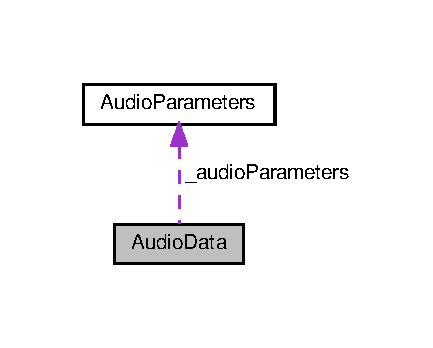
\includegraphics[width=208pt]{class_audio_data__coll__graph}
\end{center}
\end{figure}
\subsection*{Public Member Functions}
\begin{DoxyCompactItemize}
\item 
\mbox{\Hypertarget{class_audio_data_a6d84c2a7e4e8097b8925d4209fdc99a0}\label{class_audio_data_a6d84c2a7e4e8097b8925d4209fdc99a0}} 
{\bfseries Audio\+Data} (int frame\+Index, int max\+Frame\+Index)
\end{DoxyCompactItemize}
\subsection*{Public Attributes}
\begin{DoxyCompactItemize}
\item 
\mbox{\Hypertarget{class_audio_data_ae38d0347b7546de40aa981a8cbf48921}\label{class_audio_data_ae38d0347b7546de40aa981a8cbf48921}} 
int {\bfseries \+\_\+frame\+Index}
\item 
\mbox{\Hypertarget{class_audio_data_a4fa9a944e1b94479c065467d9932f8cf}\label{class_audio_data_a4fa9a944e1b94479c065467d9932f8cf}} 
int {\bfseries \+\_\+max\+Frame\+Index}
\item 
\mbox{\Hypertarget{class_audio_data_a3f83072687fa7fbf8742d65546c81336}\label{class_audio_data_a3f83072687fa7fbf8742d65546c81336}} 
float $\ast$ {\bfseries \+\_\+record\+Samples}
\item 
\mbox{\Hypertarget{class_audio_data_a248d85d55007c28b6917d99610b62560}\label{class_audio_data_a248d85d55007c28b6917d99610b62560}} 
std\+::size\+\_\+t {\bfseries \+\_\+record\+Size}
\item 
\mbox{\Hypertarget{class_audio_data_a6d9608381036a1e5a99f1f84960eb012}\label{class_audio_data_a6d9608381036a1e5a99f1f84960eb012}} 
\hyperlink{class_audio_parameters}{Audio\+Parameters} $\ast$ {\bfseries \+\_\+audio\+Parameters}
\end{DoxyCompactItemize}


The documentation for this class was generated from the following files\+:\begin{DoxyCompactItemize}
\item 
Client/include/\+Audio/Audio\+Data.\+hpp\item 
Client/src/\+Audio/Audio\+Data.\+cpp\end{DoxyCompactItemize}

\hypertarget{classbbl_1_1cli_1_1audio_1_1_audio_listener}{}\section{bbl\+:\+:cli\+:\+:audio\+:\+:Audio\+Listener Class Reference}
\label{classbbl_1_1cli_1_1audio_1_1_audio_listener}\index{bbl\+::cli\+::audio\+::\+Audio\+Listener@{bbl\+::cli\+::audio\+::\+Audio\+Listener}}


Inheritance diagram for bbl\+:\+:cli\+:\+:audio\+:\+:Audio\+Listener\+:
\nopagebreak
\begin{figure}[H]
\begin{center}
\leavevmode
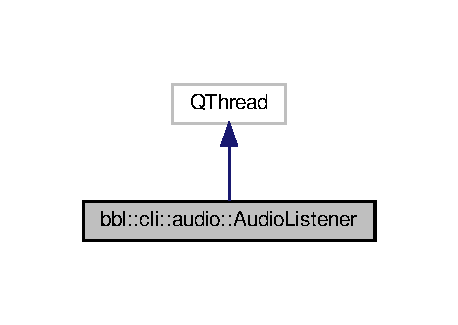
\includegraphics[width=220pt]{classbbl_1_1cli_1_1audio_1_1_audio_listener__inherit__graph}
\end{center}
\end{figure}


Collaboration diagram for bbl\+:\+:cli\+:\+:audio\+:\+:Audio\+Listener\+:
\nopagebreak
\begin{figure}[H]
\begin{center}
\leavevmode
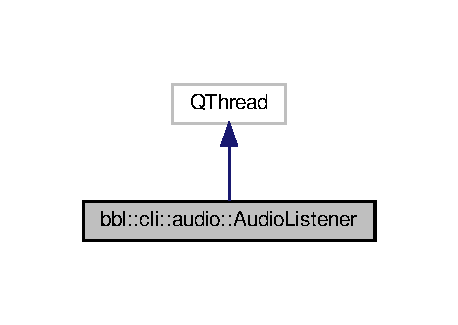
\includegraphics[width=220pt]{classbbl_1_1cli_1_1audio_1_1_audio_listener__coll__graph}
\end{center}
\end{figure}
\subsection*{Public Member Functions}
\begin{DoxyCompactItemize}
\item 
\mbox{\Hypertarget{classbbl_1_1cli_1_1audio_1_1_audio_listener_ac9340086f6765ccc17fa23209a15f388}\label{classbbl_1_1cli_1_1audio_1_1_audio_listener_ac9340086f6765ccc17fa23209a15f388}} 
{\bfseries Audio\+Listener} (\hyperlink{classbbl_1_1cli_1_1_i_udp_client}{I\+Udp\+Client} $\ast$client)
\item 
\mbox{\Hypertarget{classbbl_1_1cli_1_1audio_1_1_audio_listener_a2a01bf427f620ab8d2417c2502ebf7fb}\label{classbbl_1_1cli_1_1audio_1_1_audio_listener_a2a01bf427f620ab8d2417c2502ebf7fb}} 
void {\bfseries run} ()
\item 
\mbox{\Hypertarget{classbbl_1_1cli_1_1audio_1_1_audio_listener_a366e2bd9318fd03a8e559d809c1656c5}\label{classbbl_1_1cli_1_1audio_1_1_audio_listener_a366e2bd9318fd03a8e559d809c1656c5}} 
void {\bfseries destroy} ()
\end{DoxyCompactItemize}


The documentation for this class was generated from the following files\+:\begin{DoxyCompactItemize}
\item 
Client/include/\+Audio/Audio\+Listener.\+hpp\item 
Client/src/\+Audio/Audio\+Listener.\+cpp\end{DoxyCompactItemize}

\hypertarget{class_audio_manager}{}\section{Audio\+Manager Class Reference}
\label{class_audio_manager}\index{Audio\+Manager@{Audio\+Manager}}
\subsection*{Public Member Functions}
\begin{DoxyCompactItemize}
\item 
\mbox{\Hypertarget{class_audio_manager_a4c6081ec4f81730e4a96c36a7788ea74}\label{class_audio_manager_a4c6081ec4f81730e4a96c36a7788ea74}} 
void {\bfseries start\+Record} ()
\item 
\mbox{\Hypertarget{class_audio_manager_a30976c3f30e4c5d93904c2468fdae7b1}\label{class_audio_manager_a30976c3f30e4c5d93904c2468fdae7b1}} 
void {\bfseries play\+Record} ()
\item 
\mbox{\Hypertarget{class_audio_manager_a9bdf7b74899cc5674f0b0812ae43059d}\label{class_audio_manager_a9bdf7b74899cc5674f0b0812ae43059d}} 
float $\ast$ {\bfseries get\+Data\+Samples} () const
\item 
\mbox{\Hypertarget{class_audio_manager_a812a53f2ed8f9cf57f300b7df57a8dfb}\label{class_audio_manager_a812a53f2ed8f9cf57f300b7df57a8dfb}} 
std\+::size\+\_\+t {\bfseries get\+Size\+Samples} () const
\item 
\mbox{\Hypertarget{class_audio_manager_a12f4eea9001273f0bdb913a8e280f25f}\label{class_audio_manager_a12f4eea9001273f0bdb913a8e280f25f}} 
void {\bfseries set\+Data\+Samples} (float $\ast$data)
\end{DoxyCompactItemize}


The documentation for this class was generated from the following files\+:\begin{DoxyCompactItemize}
\item 
Client/include/\+Audio/Audio\+Manager.\+hpp\item 
Client/src/\+Audio/Audio\+Manager.\+cpp\end{DoxyCompactItemize}

\hypertarget{class_audio_parameters}{}\section{Audio\+Parameters Class Reference}
\label{class_audio_parameters}\index{Audio\+Parameters@{Audio\+Parameters}}
\subsection*{Public Member Functions}
\begin{DoxyCompactItemize}
\item 
\mbox{\Hypertarget{class_audio_parameters_aeacd7bd0438f3445886d10ce0bfa0a8c}\label{class_audio_parameters_aeacd7bd0438f3445886d10ce0bfa0a8c}} 
int {\bfseries get\+Sample\+Rate} () const
\item 
\mbox{\Hypertarget{class_audio_parameters_a89d5c68a2c997262ac5a1b93db839b6a}\label{class_audio_parameters_a89d5c68a2c997262ac5a1b93db839b6a}} 
int {\bfseries get\+Framer\+Buffer} () const
\item 
\mbox{\Hypertarget{class_audio_parameters_ae1a079b4a0dda11b07479b93e89863dc}\label{class_audio_parameters_ae1a079b4a0dda11b07479b93e89863dc}} 
float {\bfseries get\+Record\+Time} () const
\item 
\mbox{\Hypertarget{class_audio_parameters_a5be402b4ff7f30d3dc44d757ed83faba}\label{class_audio_parameters_a5be402b4ff7f30d3dc44d757ed83faba}} 
std\+::size\+\_\+t {\bfseries get\+Channel\+Number} () const
\end{DoxyCompactItemize}
\subsection*{Public Attributes}
\begin{DoxyCompactItemize}
\item 
\mbox{\Hypertarget{class_audio_parameters_aa6b0ae10ae44735a62d66ce42cbf1c42}\label{class_audio_parameters_aa6b0ae10ae44735a62d66ce42cbf1c42}} 
const int {\bfseries \+\_\+sample\+Rate}
\item 
\mbox{\Hypertarget{class_audio_parameters_af94336fef7592c3d98a5799c8556066a}\label{class_audio_parameters_af94336fef7592c3d98a5799c8556066a}} 
const int {\bfseries \+\_\+frame\+Per\+Second}
\item 
\mbox{\Hypertarget{class_audio_parameters_aa6005b4cabdf57276aa389524da17f6b}\label{class_audio_parameters_aa6005b4cabdf57276aa389524da17f6b}} 
const float {\bfseries \+\_\+record\+Time}
\item 
\mbox{\Hypertarget{class_audio_parameters_ac63e7fcdbb3231ed3a8759566229497c}\label{class_audio_parameters_ac63e7fcdbb3231ed3a8759566229497c}} 
const std\+::size\+\_\+t {\bfseries \+\_\+channel\+Number}
\end{DoxyCompactItemize}


The documentation for this class was generated from the following file\+:\begin{DoxyCompactItemize}
\item 
Client/include/\+Audio/Audio\+Parameters.\+hpp\end{DoxyCompactItemize}

\hypertarget{classbbl_1_1cli_1_1audio_1_1_audio_recorder}{}\section{bbl\+:\+:cli\+:\+:audio\+:\+:Audio\+Recorder Class Reference}
\label{classbbl_1_1cli_1_1audio_1_1_audio_recorder}\index{bbl\+::cli\+::audio\+::\+Audio\+Recorder@{bbl\+::cli\+::audio\+::\+Audio\+Recorder}}


Inheritance diagram for bbl\+:\+:cli\+:\+:audio\+:\+:Audio\+Recorder\+:
\nopagebreak
\begin{figure}[H]
\begin{center}
\leavevmode
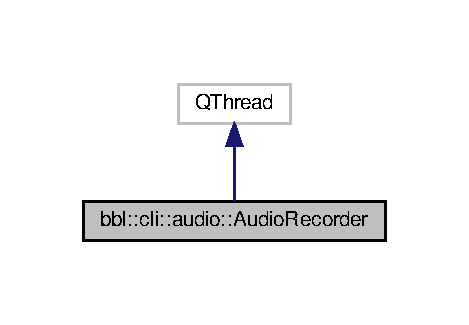
\includegraphics[width=225pt]{classbbl_1_1cli_1_1audio_1_1_audio_recorder__inherit__graph}
\end{center}
\end{figure}


Collaboration diagram for bbl\+:\+:cli\+:\+:audio\+:\+:Audio\+Recorder\+:
\nopagebreak
\begin{figure}[H]
\begin{center}
\leavevmode
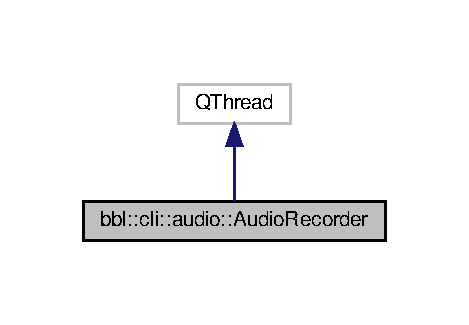
\includegraphics[width=225pt]{classbbl_1_1cli_1_1audio_1_1_audio_recorder__coll__graph}
\end{center}
\end{figure}
\subsection*{Public Member Functions}
\begin{DoxyCompactItemize}
\item 
\mbox{\Hypertarget{classbbl_1_1cli_1_1audio_1_1_audio_recorder_aab286f8a53246a44c709daf1f1059598}\label{classbbl_1_1cli_1_1audio_1_1_audio_recorder_aab286f8a53246a44c709daf1f1059598}} 
{\bfseries Audio\+Recorder} (\hyperlink{classbbl_1_1cli_1_1_i_udp_client}{I\+Udp\+Client} $\ast$client)
\item 
\mbox{\Hypertarget{classbbl_1_1cli_1_1audio_1_1_audio_recorder_adf6273d04355b7cdb0b4594bb981e759}\label{classbbl_1_1cli_1_1audio_1_1_audio_recorder_adf6273d04355b7cdb0b4594bb981e759}} 
void {\bfseries run} ()
\item 
\mbox{\Hypertarget{classbbl_1_1cli_1_1audio_1_1_audio_recorder_aa06624646e90292ba5c7ea9dcfff3cfa}\label{classbbl_1_1cli_1_1audio_1_1_audio_recorder_aa06624646e90292ba5c7ea9dcfff3cfa}} 
void {\bfseries destroy} ()
\end{DoxyCompactItemize}


The documentation for this class was generated from the following files\+:\begin{DoxyCompactItemize}
\item 
Client/include/\+Audio/Audio\+Recorder.\+hpp\item 
Client/src/\+Audio/Audio\+Recorder.\+cpp\end{DoxyCompactItemize}

\hypertarget{classbbl_1_1srv_1_1_boost_network_client}{}\section{bbl\+:\+:srv\+:\+:Boost\+Network\+Client Class Reference}
\label{classbbl_1_1srv_1_1_boost_network_client}\index{bbl\+::srv\+::\+Boost\+Network\+Client@{bbl\+::srv\+::\+Boost\+Network\+Client}}


Inheritance diagram for bbl\+:\+:srv\+:\+:Boost\+Network\+Client\+:
\nopagebreak
\begin{figure}[H]
\begin{center}
\leavevmode
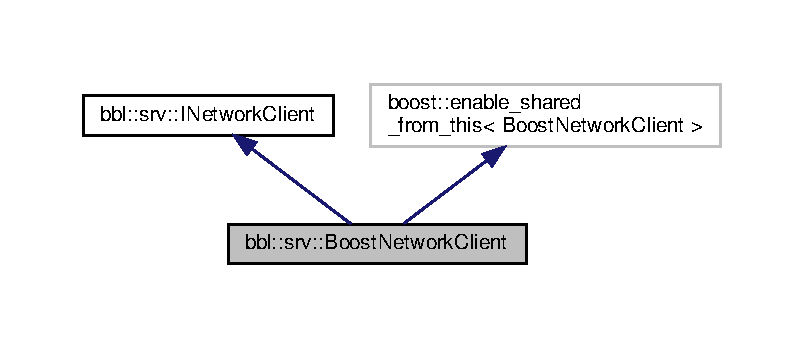
\includegraphics[width=350pt]{classbbl_1_1srv_1_1_boost_network_client__inherit__graph}
\end{center}
\end{figure}


Collaboration diagram for bbl\+:\+:srv\+:\+:Boost\+Network\+Client\+:
\nopagebreak
\begin{figure}[H]
\begin{center}
\leavevmode
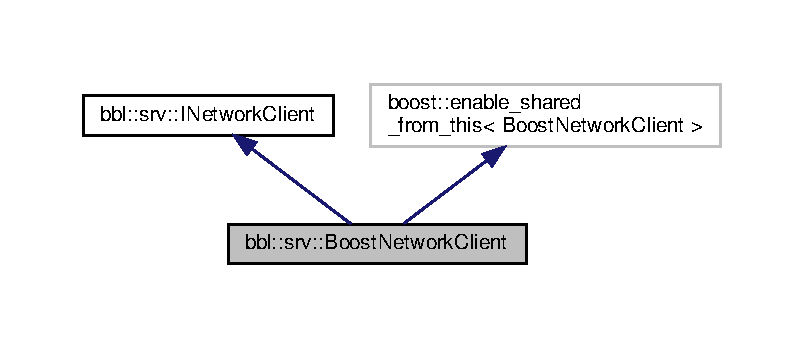
\includegraphics[width=350pt]{classbbl_1_1srv_1_1_boost_network_client__coll__graph}
\end{center}
\end{figure}
\subsection*{Public Member Functions}
\begin{DoxyCompactItemize}
\item 
\mbox{\Hypertarget{classbbl_1_1srv_1_1_boost_network_client_ac1fb8f11d0beaf53d95f23cd4d0e090c}\label{classbbl_1_1srv_1_1_boost_network_client_ac1fb8f11d0beaf53d95f23cd4d0e090c}} 
{\bfseries Boost\+Network\+Client} (basic\+\_\+socket\+\_\+acceptor$<$ tcp $>$ \&ec, \hyperlink{classbbl_1_1srv_1_1_network_manager}{Network\+Manager} \&service)
\item 
\mbox{\Hypertarget{classbbl_1_1srv_1_1_boost_network_client_abf9374c65de4a17a64f3fe2555c0290a}\label{classbbl_1_1srv_1_1_boost_network_client_abf9374c65de4a17a64f3fe2555c0290a}} 
{\bfseries Boost\+Network\+Client} (const \hyperlink{classbbl_1_1srv_1_1_boost_network_client}{Boost\+Network\+Client} \&)=delete
\item 
\mbox{\Hypertarget{classbbl_1_1srv_1_1_boost_network_client_ab68bde7428536219fa926cd514741406}\label{classbbl_1_1srv_1_1_boost_network_client_ab68bde7428536219fa926cd514741406}} 
\hyperlink{classbbl_1_1srv_1_1_boost_network_client}{Boost\+Network\+Client} \& {\bfseries operator=} (const \hyperlink{classbbl_1_1srv_1_1_boost_network_client}{Boost\+Network\+Client} \&)=delete
\item 
\mbox{\Hypertarget{classbbl_1_1srv_1_1_boost_network_client_a72406d7c6c06d2da24c83415645d309e}\label{classbbl_1_1srv_1_1_boost_network_client_a72406d7c6c06d2da24c83415645d309e}} 
void {\bfseries send} (const std\+::string \&data)
\item 
\mbox{\Hypertarget{classbbl_1_1srv_1_1_boost_network_client_a5ee43cb5d04b84d98193ee1f162036e3}\label{classbbl_1_1srv_1_1_boost_network_client_a5ee43cb5d04b84d98193ee1f162036e3}} 
tcp\+::socket \& {\bfseries get\+Socket} ()
\item 
\mbox{\Hypertarget{classbbl_1_1srv_1_1_boost_network_client_a7fdbcb32b3add5542922a37b7514a866}\label{classbbl_1_1srv_1_1_boost_network_client_a7fdbcb32b3add5542922a37b7514a866}} 
void {\bfseries bind\+Read} ()
\item 
\mbox{\Hypertarget{classbbl_1_1srv_1_1_boost_network_client_ab9709338ea93ed1d02e67ada3a805adf}\label{classbbl_1_1srv_1_1_boost_network_client_ab9709338ea93ed1d02e67ada3a805adf}} 
std\+::size\+\_\+t {\bfseries get\+Id} () const
\item 
\mbox{\Hypertarget{classbbl_1_1srv_1_1_boost_network_client_a065acdf4084b7a8661c973df24f1459f}\label{classbbl_1_1srv_1_1_boost_network_client_a065acdf4084b7a8661c973df24f1459f}} 
void {\bfseries disconnect} (const std\+::string \&message)
\item 
\mbox{\Hypertarget{classbbl_1_1srv_1_1_boost_network_client_a1712dcdcde5eb945e608a31d4d87f043}\label{classbbl_1_1srv_1_1_boost_network_client_a1712dcdcde5eb945e608a31d4d87f043}} 
void {\bfseries read\+Handler} (const boost\+::system\+::error\+\_\+code \&error, std\+::size\+\_\+t bytes\+\_\+transferred)
\item 
\mbox{\Hypertarget{classbbl_1_1srv_1_1_boost_network_client_af279e06f5fccad98e4e3d122378e04ce}\label{classbbl_1_1srv_1_1_boost_network_client_af279e06f5fccad98e4e3d122378e04ce}} 
void {\bfseries write\+Handler} (const boost\+::system\+::error\+\_\+code \&error, std\+::size\+\_\+t bytes\+\_\+transferred)
\end{DoxyCompactItemize}


The documentation for this class was generated from the following files\+:\begin{DoxyCompactItemize}
\item 
Server/include/\+Network/Boost\+Network\+Client.\+hpp\item 
Server/src/\+Network/Boost\+Network\+Client.\+cpp\end{DoxyCompactItemize}

\hypertarget{classbbl_1_1srv_1_1_boost_network_server}{}\section{bbl\+:\+:srv\+:\+:Boost\+Network\+Server Class Reference}
\label{classbbl_1_1srv_1_1_boost_network_server}\index{bbl\+::srv\+::\+Boost\+Network\+Server@{bbl\+::srv\+::\+Boost\+Network\+Server}}


Inheritance diagram for bbl\+:\+:srv\+:\+:Boost\+Network\+Server\+:
\nopagebreak
\begin{figure}[H]
\begin{center}
\leavevmode
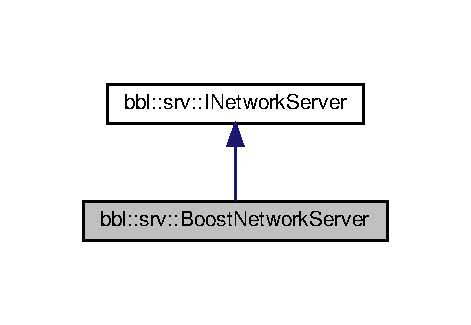
\includegraphics[width=226pt]{classbbl_1_1srv_1_1_boost_network_server__inherit__graph}
\end{center}
\end{figure}


Collaboration diagram for bbl\+:\+:srv\+:\+:Boost\+Network\+Server\+:
\nopagebreak
\begin{figure}[H]
\begin{center}
\leavevmode
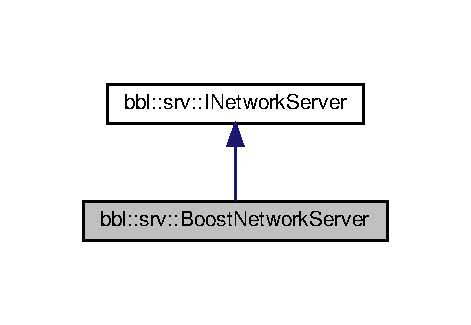
\includegraphics[width=226pt]{classbbl_1_1srv_1_1_boost_network_server__coll__graph}
\end{center}
\end{figure}
\subsection*{Public Member Functions}
\begin{DoxyCompactItemize}
\item 
\mbox{\Hypertarget{classbbl_1_1srv_1_1_boost_network_server_a6831661826ea6906ddd798ec3414294a}\label{classbbl_1_1srv_1_1_boost_network_server_a6831661826ea6906ddd798ec3414294a}} 
{\bfseries Boost\+Network\+Server} (unsigned short port, \hyperlink{classbbl_1_1srv_1_1_network_manager}{Network\+Manager} \&service)
\item 
\mbox{\Hypertarget{classbbl_1_1srv_1_1_boost_network_server_ab909811fb953a738a7ae537d16054100}\label{classbbl_1_1srv_1_1_boost_network_server_ab909811fb953a738a7ae537d16054100}} 
{\bfseries Boost\+Network\+Server} (const \hyperlink{classbbl_1_1srv_1_1_boost_network_server}{Boost\+Network\+Server} \&)=delete
\item 
\mbox{\Hypertarget{classbbl_1_1srv_1_1_boost_network_server_a26870afa82287b1dc2f63ec076970738}\label{classbbl_1_1srv_1_1_boost_network_server_a26870afa82287b1dc2f63ec076970738}} 
\hyperlink{classbbl_1_1srv_1_1_boost_network_server}{Boost\+Network\+Server} \& {\bfseries operator=} (const \hyperlink{classbbl_1_1srv_1_1_boost_network_server}{Boost\+Network\+Server} \&)=delete
\item 
\mbox{\Hypertarget{classbbl_1_1srv_1_1_boost_network_server_a76142867d491aa36761ef8fe76d6ec36}\label{classbbl_1_1srv_1_1_boost_network_server_a76142867d491aa36761ef8fe76d6ec36}} 
void {\bfseries run} ()
\end{DoxyCompactItemize}


The documentation for this class was generated from the following files\+:\begin{DoxyCompactItemize}
\item 
Server/include/\+Network/Boost\+Network\+Server.\+hpp\item 
Server/src/\+Network/Boost\+Network\+Server.\+cpp\end{DoxyCompactItemize}

\hypertarget{classbbl_1_1cli_1_1_boost_tcp_client}{}\section{bbl\+:\+:cli\+:\+:Boost\+Tcp\+Client Class Reference}
\label{classbbl_1_1cli_1_1_boost_tcp_client}\index{bbl\+::cli\+::\+Boost\+Tcp\+Client@{bbl\+::cli\+::\+Boost\+Tcp\+Client}}


Inheritance diagram for bbl\+:\+:cli\+:\+:Boost\+Tcp\+Client\+:
\nopagebreak
\begin{figure}[H]
\begin{center}
\leavevmode
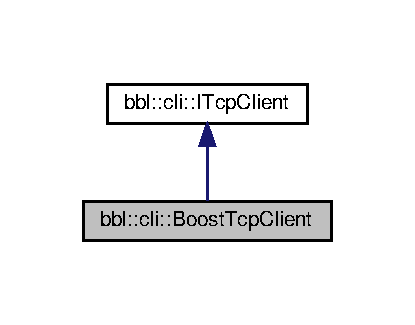
\includegraphics[width=199pt]{classbbl_1_1cli_1_1_boost_tcp_client__inherit__graph}
\end{center}
\end{figure}


Collaboration diagram for bbl\+:\+:cli\+:\+:Boost\+Tcp\+Client\+:
\nopagebreak
\begin{figure}[H]
\begin{center}
\leavevmode
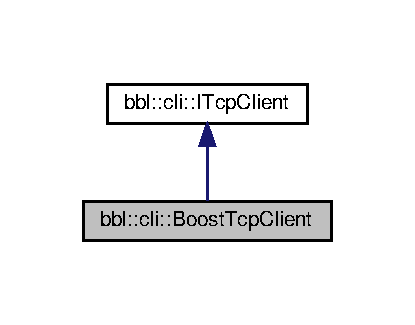
\includegraphics[width=199pt]{classbbl_1_1cli_1_1_boost_tcp_client__coll__graph}
\end{center}
\end{figure}
\subsection*{Public Member Functions}
\begin{DoxyCompactItemize}
\item 
\mbox{\Hypertarget{classbbl_1_1cli_1_1_boost_tcp_client_a7fc15f3bd8362810778c399d6287947c}\label{classbbl_1_1cli_1_1_boost_tcp_client_a7fc15f3bd8362810778c399d6287947c}} 
{\bfseries Boost\+Tcp\+Client} (const std\+::string \&ipv4, unsigned short port)
\item 
\mbox{\Hypertarget{classbbl_1_1cli_1_1_boost_tcp_client_ab293037b6a6e4da6bbafc7db3b400333}\label{classbbl_1_1cli_1_1_boost_tcp_client_ab293037b6a6e4da6bbafc7db3b400333}} 
{\bfseries Boost\+Tcp\+Client} (const \hyperlink{classbbl_1_1cli_1_1_boost_tcp_client}{Boost\+Tcp\+Client} \&)=delete
\item 
\mbox{\Hypertarget{classbbl_1_1cli_1_1_boost_tcp_client_a4492d638ef5c41c65ade72a408a03bbd}\label{classbbl_1_1cli_1_1_boost_tcp_client_a4492d638ef5c41c65ade72a408a03bbd}} 
\hyperlink{classbbl_1_1cli_1_1_boost_tcp_client}{Boost\+Tcp\+Client} \& {\bfseries operator=} (const \hyperlink{classbbl_1_1cli_1_1_boost_tcp_client}{Boost\+Tcp\+Client} \&)=delete
\item 
\mbox{\Hypertarget{classbbl_1_1cli_1_1_boost_tcp_client_ac2dee8492cf958fa1f10c19ac9b68919}\label{classbbl_1_1cli_1_1_boost_tcp_client_ac2dee8492cf958fa1f10c19ac9b68919}} 
void {\bfseries send} (const std\+::string \&data)
\item 
\mbox{\Hypertarget{classbbl_1_1cli_1_1_boost_tcp_client_a238e3f918d949353a8145d42f46d231c}\label{classbbl_1_1cli_1_1_boost_tcp_client_a238e3f918d949353a8145d42f46d231c}} 
std\+::string {\bfseries recv} ()
\end{DoxyCompactItemize}


The documentation for this class was generated from the following files\+:\begin{DoxyCompactItemize}
\item 
Client/include/\+Network/Boost\+Tcp\+Client.\+hpp\item 
Client/src/\+Network/Boost\+Tcp\+Client.\+cpp\end{DoxyCompactItemize}

\hypertarget{classbbl_1_1cli_1_1_boost_udp_client}{}\section{bbl\+:\+:cli\+:\+:Boost\+Udp\+Client Class Reference}
\label{classbbl_1_1cli_1_1_boost_udp_client}\index{bbl\+::cli\+::\+Boost\+Udp\+Client@{bbl\+::cli\+::\+Boost\+Udp\+Client}}


Inheritance diagram for bbl\+:\+:cli\+:\+:Boost\+Udp\+Client\+:
\nopagebreak
\begin{figure}[H]
\begin{center}
\leavevmode
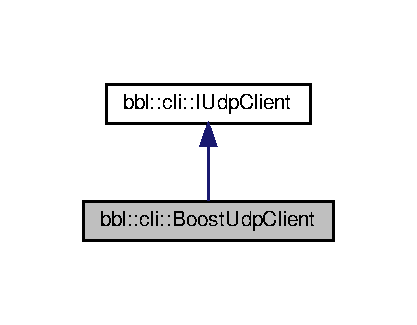
\includegraphics[width=200pt]{classbbl_1_1cli_1_1_boost_udp_client__inherit__graph}
\end{center}
\end{figure}


Collaboration diagram for bbl\+:\+:cli\+:\+:Boost\+Udp\+Client\+:
\nopagebreak
\begin{figure}[H]
\begin{center}
\leavevmode
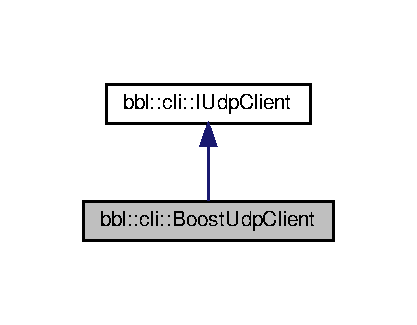
\includegraphics[width=200pt]{classbbl_1_1cli_1_1_boost_udp_client__coll__graph}
\end{center}
\end{figure}
\subsection*{Public Member Functions}
\begin{DoxyCompactItemize}
\item 
\mbox{\Hypertarget{classbbl_1_1cli_1_1_boost_udp_client_af207eb99cc70e7c41baacdbab0e07e80}\label{classbbl_1_1cli_1_1_boost_udp_client_af207eb99cc70e7c41baacdbab0e07e80}} 
{\bfseries Boost\+Udp\+Client} (const std\+::string \&ipv4, unsigned short port, bool is\+\_\+receiver)
\item 
\mbox{\Hypertarget{classbbl_1_1cli_1_1_boost_udp_client_aa2d49a11b5a4d645c137544c2264eb09}\label{classbbl_1_1cli_1_1_boost_udp_client_aa2d49a11b5a4d645c137544c2264eb09}} 
{\bfseries Boost\+Udp\+Client} (const \hyperlink{classbbl_1_1cli_1_1_boost_udp_client}{Boost\+Udp\+Client} \&)=delete
\item 
\mbox{\Hypertarget{classbbl_1_1cli_1_1_boost_udp_client_a91b9cf1dfadec551e69a8a74407a0383}\label{classbbl_1_1cli_1_1_boost_udp_client_a91b9cf1dfadec551e69a8a74407a0383}} 
\hyperlink{classbbl_1_1cli_1_1_boost_udp_client}{Boost\+Udp\+Client} \& {\bfseries operator=} (const \hyperlink{classbbl_1_1cli_1_1_boost_udp_client}{Boost\+Udp\+Client} \&)=delete
\item 
\mbox{\Hypertarget{classbbl_1_1cli_1_1_boost_udp_client_a4dc85825ff44f877ebf686f52639ce2d}\label{classbbl_1_1cli_1_1_boost_udp_client_a4dc85825ff44f877ebf686f52639ce2d}} 
void {\bfseries send} (const \hyperlink{classbbl_1_1cli_1_1_packet}{Packet} \&packet)
\item 
\mbox{\Hypertarget{classbbl_1_1cli_1_1_boost_udp_client_acb133442fe8501c05ceb918153c3fe75}\label{classbbl_1_1cli_1_1_boost_udp_client_acb133442fe8501c05ceb918153c3fe75}} 
\hyperlink{classbbl_1_1cli_1_1_packet}{Packet} {\bfseries recv} ()
\item 
\mbox{\Hypertarget{classbbl_1_1cli_1_1_boost_udp_client_a50bf4567a00e5eaeddb4ab0b2f03b7ce}\label{classbbl_1_1cli_1_1_boost_udp_client_a50bf4567a00e5eaeddb4ab0b2f03b7ce}} 
unsigned short {\bfseries get\+Port} () const
\item 
\mbox{\Hypertarget{classbbl_1_1cli_1_1_boost_udp_client_a085689d1413a8f8c78a245475b56f931}\label{classbbl_1_1cli_1_1_boost_udp_client_a085689d1413a8f8c78a245475b56f931}} 
std\+::string {\bfseries get\+Address} () const
\item 
\mbox{\Hypertarget{classbbl_1_1cli_1_1_boost_udp_client_aa484ce9f37376d6efca4585cbe42fe6d}\label{classbbl_1_1cli_1_1_boost_udp_client_aa484ce9f37376d6efca4585cbe42fe6d}} 
void {\bfseries close} ()
\end{DoxyCompactItemize}


The documentation for this class was generated from the following files\+:\begin{DoxyCompactItemize}
\item 
Client/include/\+Network/Boost\+Udp\+Client.\+hpp\item 
Client/src/\+Network/Boost\+Udp\+Client.\+cpp\end{DoxyCompactItemize}

\hypertarget{classbbl_1_1cli_1_1_client}{}\section{bbl\+:\+:cli\+:\+:Client Class Reference}
\label{classbbl_1_1cli_1_1_client}\index{bbl\+::cli\+::\+Client@{bbl\+::cli\+::\+Client}}
\subsection*{Public Member Functions}
\begin{DoxyCompactItemize}
\item 
\mbox{\Hypertarget{classbbl_1_1cli_1_1_client_ab5ab3a77c84e5bc39dc653cef343b8ac}\label{classbbl_1_1cli_1_1_client_ab5ab3a77c84e5bc39dc653cef343b8ac}} 
{\bfseries Client} (\hyperlink{classbbl_1_1cli_1_1_i_tcp_client}{I\+Tcp\+Client} $\ast$tcp\+Connection)
\item 
\mbox{\Hypertarget{classbbl_1_1cli_1_1_client_acfc496485b229bd8c2af8d5492f16c3f}\label{classbbl_1_1cli_1_1_client_acfc496485b229bd8c2af8d5492f16c3f}} 
{\bfseries Client} (const \hyperlink{classbbl_1_1cli_1_1_client}{Client} \&)=delete
\item 
\mbox{\Hypertarget{classbbl_1_1cli_1_1_client_abd2ba96ec1ebdbbf67836257dc683332}\label{classbbl_1_1cli_1_1_client_abd2ba96ec1ebdbbf67836257dc683332}} 
\hyperlink{classbbl_1_1cli_1_1_client}{Client} \& {\bfseries operator=} (const \hyperlink{classbbl_1_1cli_1_1_client}{Client} \&)=delete
\item 
\mbox{\Hypertarget{classbbl_1_1cli_1_1_client_afcbe6046c74e86b64c1b861f5e58ffbd}\label{classbbl_1_1cli_1_1_client_afcbe6046c74e86b64c1b861f5e58ffbd}} 
bool {\bfseries is\+Logged} () const
\item 
\mbox{\Hypertarget{classbbl_1_1cli_1_1_client_afecc09190f29820f373b35b13f42338c}\label{classbbl_1_1cli_1_1_client_afecc09190f29820f373b35b13f42338c}} 
void {\bfseries registration} (const std\+::string \&username, const std\+::string \&password)
\item 
\mbox{\Hypertarget{classbbl_1_1cli_1_1_client_abf1626c0fd720a8ba69b811b718411da}\label{classbbl_1_1cli_1_1_client_abf1626c0fd720a8ba69b811b718411da}} 
void {\bfseries login} (const std\+::string \&username, const std\+::string \&password)
\item 
\mbox{\Hypertarget{classbbl_1_1cli_1_1_client_aa977795294407c10fe843b5bc28b6685}\label{classbbl_1_1cli_1_1_client_aa977795294407c10fe843b5bc28b6685}} 
void {\bfseries logout} ()
\item 
\mbox{\Hypertarget{classbbl_1_1cli_1_1_client_af2df5e5c39d2d109a3a0efdc7db110b8}\label{classbbl_1_1cli_1_1_client_af2df5e5c39d2d109a3a0efdc7db110b8}} 
void {\bfseries request\+Invitation} (const std\+::string \&contact)
\item 
\mbox{\Hypertarget{classbbl_1_1cli_1_1_client_affd3e03b029a61eb0a090cdc059538ec}\label{classbbl_1_1cli_1_1_client_affd3e03b029a61eb0a090cdc059538ec}} 
void {\bfseries accept\+Invitation} (const std\+::string \&contact)
\item 
\mbox{\Hypertarget{classbbl_1_1cli_1_1_client_a1a53802b4412dbb0373e56258b91daab}\label{classbbl_1_1cli_1_1_client_a1a53802b4412dbb0373e56258b91daab}} 
std\+::vector$<$ std\+::string $>$ {\bfseries get\+Invitations} ()
\item 
\mbox{\Hypertarget{classbbl_1_1cli_1_1_client_ae87912ca10ad9f26abeeccc41f24712f}\label{classbbl_1_1cli_1_1_client_ae87912ca10ad9f26abeeccc41f24712f}} 
std\+::vector$<$ std\+::string $>$ {\bfseries get\+Contacts} ()
\item 
\mbox{\Hypertarget{classbbl_1_1cli_1_1_client_a293eae6663d07bd1d95a04a49b712bfb}\label{classbbl_1_1cli_1_1_client_a293eae6663d07bd1d95a04a49b712bfb}} 
void {\bfseries set\+Udp\+Setting} (const std\+::string \&ipv4, unsigned short port)
\item 
\mbox{\Hypertarget{classbbl_1_1cli_1_1_client_aa3bb631819f71fd2f0423dd6dc410068}\label{classbbl_1_1cli_1_1_client_aa3bb631819f71fd2f0423dd6dc410068}} 
std\+::pair$<$ std\+::string, unsigned short $>$ {\bfseries get\+Udp\+Settings} (const std\+::string \&contact)
\end{DoxyCompactItemize}


The documentation for this class was generated from the following files\+:\begin{DoxyCompactItemize}
\item 
Client/include/\+Core/Client.\+hpp\item 
Client/src/\+Core/Client.\+cpp\end{DoxyCompactItemize}

\hypertarget{classbbl_1_1srv_1_1_command_parser}{}\section{bbl\+:\+:srv\+:\+:Command\+Parser Class Reference}
\label{classbbl_1_1srv_1_1_command_parser}\index{bbl\+::srv\+::\+Command\+Parser@{bbl\+::srv\+::\+Command\+Parser}}
\subsection*{Static Public Member Functions}
\begin{DoxyCompactItemize}
\item 
\mbox{\Hypertarget{classbbl_1_1srv_1_1_command_parser_ac6860168a27117589bf4fd07a5177e97}\label{classbbl_1_1srv_1_1_command_parser_ac6860168a27117589bf4fd07a5177e97}} 
static void {\bfseries parse} (std\+::vector$<$ \hyperlink{classbbl_1_1srv_1_1_user}{User} $\ast$$>$ \+\_\+clients, \hyperlink{classbbl_1_1srv_1_1_user}{User} $\ast$current, \hyperlink{classbbl_1_1srv_1_1_i_storage}{I\+Storage} $\ast$db, const std\+::string \&text)
\end{DoxyCompactItemize}


The documentation for this class was generated from the following files\+:\begin{DoxyCompactItemize}
\item 
Server/include/\+Core/Command\+Parser.\+hpp\item 
Server/src/\+Core/Command\+Parser.\+cpp\end{DoxyCompactItemize}

\hypertarget{classbbl_1_1srv_1_1_contact_list_command}{}\section{bbl\+:\+:srv\+:\+:Contact\+List\+Command Class Reference}
\label{classbbl_1_1srv_1_1_contact_list_command}\index{bbl\+::srv\+::\+Contact\+List\+Command@{bbl\+::srv\+::\+Contact\+List\+Command}}
\subsection*{Static Public Member Functions}
\begin{DoxyCompactItemize}
\item 
\mbox{\Hypertarget{classbbl_1_1srv_1_1_contact_list_command_a4e7abf48164a6b1d3c294ddb17eb8618}\label{classbbl_1_1srv_1_1_contact_list_command_a4e7abf48164a6b1d3c294ddb17eb8618}} 
static void {\bfseries run} (std\+::vector$<$ \hyperlink{classbbl_1_1srv_1_1_user}{User} $\ast$$>$ \+\_\+clients, \hyperlink{classbbl_1_1srv_1_1_user}{User} $\ast$current, \hyperlink{classbbl_1_1srv_1_1_i_storage}{I\+Storage} $\ast$db, const std\+::vector$<$ std\+::string $>$ \&av)
\end{DoxyCompactItemize}


The documentation for this class was generated from the following file\+:\begin{DoxyCompactItemize}
\item 
Server/include/\+Core/Contact\+List\+Command.\+hpp\end{DoxyCompactItemize}

\hypertarget{classbbl_1_1cli_1_1graphics_1_1_contacts}{}\section{bbl\+:\+:cli\+:\+:graphics\+:\+:Contacts Class Reference}
\label{classbbl_1_1cli_1_1graphics_1_1_contacts}\index{bbl\+::cli\+::graphics\+::\+Contacts@{bbl\+::cli\+::graphics\+::\+Contacts}}


Inheritance diagram for bbl\+:\+:cli\+:\+:graphics\+:\+:Contacts\+:
\nopagebreak
\begin{figure}[H]
\begin{center}
\leavevmode
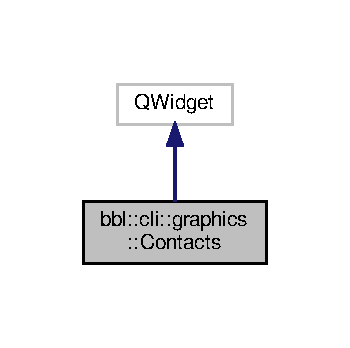
\includegraphics[width=168pt]{classbbl_1_1cli_1_1graphics_1_1_contacts__inherit__graph}
\end{center}
\end{figure}


Collaboration diagram for bbl\+:\+:cli\+:\+:graphics\+:\+:Contacts\+:
\nopagebreak
\begin{figure}[H]
\begin{center}
\leavevmode
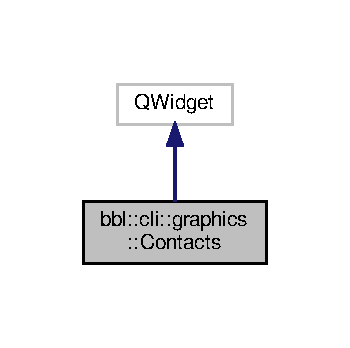
\includegraphics[width=168pt]{classbbl_1_1cli_1_1graphics_1_1_contacts__coll__graph}
\end{center}
\end{figure}
\subsection*{Public Slots}
\begin{DoxyCompactItemize}
\item 
\mbox{\Hypertarget{classbbl_1_1cli_1_1graphics_1_1_contacts_a0fbe75c5e15075b29588798cdc486dce}\label{classbbl_1_1cli_1_1graphics_1_1_contacts_a0fbe75c5e15075b29588798cdc486dce}} 
void {\bfseries refresh\+Contacts} ()
\item 
\mbox{\Hypertarget{classbbl_1_1cli_1_1graphics_1_1_contacts_a652b388e1900c2cae9026479d672e14b}\label{classbbl_1_1cli_1_1graphics_1_1_contacts_a652b388e1900c2cae9026479d672e14b}} 
void {\bfseries refresh\+Invitations} ()
\item 
\mbox{\Hypertarget{classbbl_1_1cli_1_1graphics_1_1_contacts_a26fa213a7daa06e1efb4bafe7d7dfca5}\label{classbbl_1_1cli_1_1graphics_1_1_contacts_a26fa213a7daa06e1efb4bafe7d7dfca5}} 
void {\bfseries accept\+Invitation} ()
\item 
\mbox{\Hypertarget{classbbl_1_1cli_1_1graphics_1_1_contacts_aa5659455a94a881f4082785969eae9a6}\label{classbbl_1_1cli_1_1graphics_1_1_contacts_aa5659455a94a881f4082785969eae9a6}} 
void {\bfseries call} ()
\item 
\mbox{\Hypertarget{classbbl_1_1cli_1_1graphics_1_1_contacts_ac882230cad3f0585e536ffcd3a158882}\label{classbbl_1_1cli_1_1graphics_1_1_contacts_ac882230cad3f0585e536ffcd3a158882}} 
void {\bfseries invite} ()
\end{DoxyCompactItemize}
\subsection*{Public Member Functions}
\begin{DoxyCompactItemize}
\item 
\mbox{\Hypertarget{classbbl_1_1cli_1_1graphics_1_1_contacts_a35a81d6f0ca8bad4d0f5639428450b29}\label{classbbl_1_1cli_1_1graphics_1_1_contacts_a35a81d6f0ca8bad4d0f5639428450b29}} 
{\bfseries Contacts} (Q\+Main\+Window $\ast$parent, const std\+::string \&my\+Ipv4)
\item 
\mbox{\Hypertarget{classbbl_1_1cli_1_1graphics_1_1_contacts_aedb4583a8dc30861d89e6f28ead2f46a}\label{classbbl_1_1cli_1_1graphics_1_1_contacts_aedb4583a8dc30861d89e6f28ead2f46a}} 
void {\bfseries destroy} ()
\end{DoxyCompactItemize}


The documentation for this class was generated from the following files\+:\begin{DoxyCompactItemize}
\item 
Client/include/\+Graphic/Contacts.\+hpp\item 
Client/src/\+Graphic/Contacts.\+cpp\end{DoxyCompactItemize}

\hypertarget{classbbl_1_1srv_1_1_get_invite_command}{}\section{bbl\+:\+:srv\+:\+:Get\+Invite\+Command Class Reference}
\label{classbbl_1_1srv_1_1_get_invite_command}\index{bbl\+::srv\+::\+Get\+Invite\+Command@{bbl\+::srv\+::\+Get\+Invite\+Command}}
\subsection*{Static Public Member Functions}
\begin{DoxyCompactItemize}
\item 
\mbox{\Hypertarget{classbbl_1_1srv_1_1_get_invite_command_a081c78fd4d4522ccb8b28efb3a388fb6}\label{classbbl_1_1srv_1_1_get_invite_command_a081c78fd4d4522ccb8b28efb3a388fb6}} 
static void {\bfseries run} (std\+::vector$<$ \hyperlink{classbbl_1_1srv_1_1_user}{User} $\ast$$>$ \+\_\+clients, \hyperlink{classbbl_1_1srv_1_1_user}{User} $\ast$current, \hyperlink{classbbl_1_1srv_1_1_i_storage}{I\+Storage} $\ast$db, const std\+::vector$<$ std\+::string $>$ \&av)
\end{DoxyCompactItemize}


The documentation for this class was generated from the following file\+:\begin{DoxyCompactItemize}
\item 
Server/include/\+Core/Get\+Invite\+Command.\+hpp\end{DoxyCompactItemize}

\hypertarget{classbbl_1_1srv_1_1_get_udp_command}{}\section{bbl\+:\+:srv\+:\+:Get\+Udp\+Command Class Reference}
\label{classbbl_1_1srv_1_1_get_udp_command}\index{bbl\+::srv\+::\+Get\+Udp\+Command@{bbl\+::srv\+::\+Get\+Udp\+Command}}
\subsection*{Static Public Member Functions}
\begin{DoxyCompactItemize}
\item 
\mbox{\Hypertarget{classbbl_1_1srv_1_1_get_udp_command_a155256d66ff3fc904e6be9de63a70e98}\label{classbbl_1_1srv_1_1_get_udp_command_a155256d66ff3fc904e6be9de63a70e98}} 
static void {\bfseries run} (std\+::vector$<$ \hyperlink{classbbl_1_1srv_1_1_user}{User} $\ast$$>$ \+\_\+clients, \hyperlink{classbbl_1_1srv_1_1_user}{User} $\ast$current, \hyperlink{classbbl_1_1srv_1_1_i_storage}{I\+Storage} $\ast$db, const std\+::vector$<$ std\+::string $>$ \&av)
\end{DoxyCompactItemize}


The documentation for this class was generated from the following file\+:\begin{DoxyCompactItemize}
\item 
Server/include/\+Core/Get\+Udp\+Command.\+hpp\end{DoxyCompactItemize}

\hypertarget{class_i_input}{}\section{I\+Input Class Reference}
\label{class_i_input}\index{I\+Input@{I\+Input}}


Inheritance diagram for I\+Input\+:
\nopagebreak
\begin{figure}[H]
\begin{center}
\leavevmode
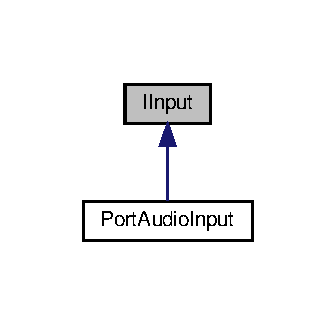
\includegraphics[width=161pt]{class_i_input__inherit__graph}
\end{center}
\end{figure}


The documentation for this class was generated from the following file\+:\begin{DoxyCompactItemize}
\item 
Client/include/\+Audio/I\+Input.\+hpp\end{DoxyCompactItemize}

\hypertarget{classbbl_1_1srv_1_1_i_network_client}{}\section{bbl\+:\+:srv\+:\+:I\+Network\+Client Class Reference}
\label{classbbl_1_1srv_1_1_i_network_client}\index{bbl\+::srv\+::\+I\+Network\+Client@{bbl\+::srv\+::\+I\+Network\+Client}}


Inheritance diagram for bbl\+:\+:srv\+:\+:I\+Network\+Client\+:
\nopagebreak
\begin{figure}[H]
\begin{center}
\leavevmode
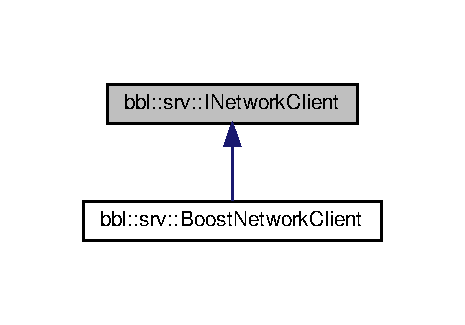
\includegraphics[width=223pt]{classbbl_1_1srv_1_1_i_network_client__inherit__graph}
\end{center}
\end{figure}
\subsection*{Public Member Functions}
\begin{DoxyCompactItemize}
\item 
\mbox{\Hypertarget{classbbl_1_1srv_1_1_i_network_client_a54d56630a807c03ffa8095299af90cc4}\label{classbbl_1_1srv_1_1_i_network_client_a54d56630a807c03ffa8095299af90cc4}} 
virtual void {\bfseries send} (const std\+::string \&data)=0
\item 
\mbox{\Hypertarget{classbbl_1_1srv_1_1_i_network_client_a7cae0fd649ec77fb2a7ff29e4288b916}\label{classbbl_1_1srv_1_1_i_network_client_a7cae0fd649ec77fb2a7ff29e4288b916}} 
virtual std\+::size\+\_\+t {\bfseries get\+Id} () const =0
\end{DoxyCompactItemize}


The documentation for this class was generated from the following file\+:\begin{DoxyCompactItemize}
\item 
Server/include/\+Network/I\+Network\+Client.\+hpp\end{DoxyCompactItemize}

\hypertarget{classbbl_1_1srv_1_1_i_network_server}{}\section{bbl\+:\+:srv\+:\+:I\+Network\+Server Class Reference}
\label{classbbl_1_1srv_1_1_i_network_server}\index{bbl\+::srv\+::\+I\+Network\+Server@{bbl\+::srv\+::\+I\+Network\+Server}}


Inheritance diagram for bbl\+:\+:srv\+:\+:I\+Network\+Server\+:
\nopagebreak
\begin{figure}[H]
\begin{center}
\leavevmode
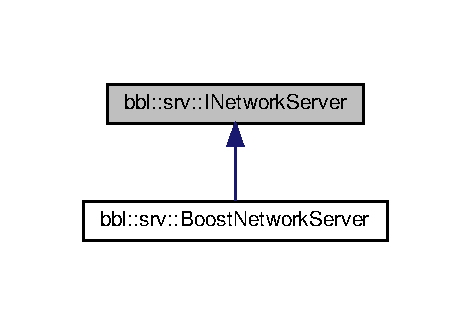
\includegraphics[width=226pt]{classbbl_1_1srv_1_1_i_network_server__inherit__graph}
\end{center}
\end{figure}
\subsection*{Public Member Functions}
\begin{DoxyCompactItemize}
\item 
\mbox{\Hypertarget{classbbl_1_1srv_1_1_i_network_server_a6d7c457c97a68f96e3d43840fbd96d12}\label{classbbl_1_1srv_1_1_i_network_server_a6d7c457c97a68f96e3d43840fbd96d12}} 
virtual void {\bfseries run} ()=0
\end{DoxyCompactItemize}


The documentation for this class was generated from the following file\+:\begin{DoxyCompactItemize}
\item 
Server/include/\+Network/I\+Network\+Server.\+hpp\end{DoxyCompactItemize}

\hypertarget{classbbl_1_1srv_1_1_invite_command}{}\section{bbl\+:\+:srv\+:\+:Invite\+Command Class Reference}
\label{classbbl_1_1srv_1_1_invite_command}\index{bbl\+::srv\+::\+Invite\+Command@{bbl\+::srv\+::\+Invite\+Command}}
\subsection*{Static Public Member Functions}
\begin{DoxyCompactItemize}
\item 
\mbox{\Hypertarget{classbbl_1_1srv_1_1_invite_command_a85c970e6e41c2f41d9ecad263a98dcbe}\label{classbbl_1_1srv_1_1_invite_command_a85c970e6e41c2f41d9ecad263a98dcbe}} 
static void {\bfseries run} (std\+::vector$<$ \hyperlink{classbbl_1_1srv_1_1_user}{User} $\ast$$>$ \+\_\+clients, \hyperlink{classbbl_1_1srv_1_1_user}{User} $\ast$current, \hyperlink{classbbl_1_1srv_1_1_i_storage}{I\+Storage} $\ast$db, const std\+::vector$<$ std\+::string $>$ \&av)
\end{DoxyCompactItemize}


The documentation for this class was generated from the following file\+:\begin{DoxyCompactItemize}
\item 
Server/include/\+Core/Invite\+Command.\+hpp\end{DoxyCompactItemize}

\hypertarget{class_i_output}{}\section{I\+Output Class Reference}
\label{class_i_output}\index{I\+Output@{I\+Output}}


Inheritance diagram for I\+Output\+:
\nopagebreak
\begin{figure}[H]
\begin{center}
\leavevmode
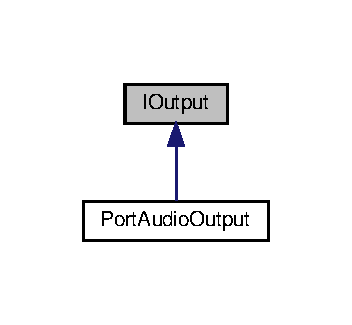
\includegraphics[width=169pt]{class_i_output__inherit__graph}
\end{center}
\end{figure}


The documentation for this class was generated from the following file\+:\begin{DoxyCompactItemize}
\item 
Client/include/\+Audio/I\+Output.\+hpp\end{DoxyCompactItemize}

\hypertarget{class_i_port_audio}{}\section{I\+Port\+Audio Class Reference}
\label{class_i_port_audio}\index{I\+Port\+Audio@{I\+Port\+Audio}}


Inheritance diagram for I\+Port\+Audio\+:
\nopagebreak
\begin{figure}[H]
\begin{center}
\leavevmode
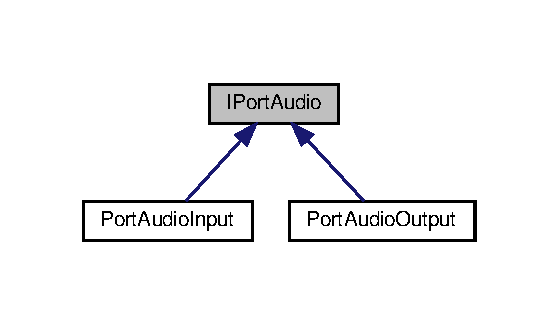
\includegraphics[width=268pt]{class_i_port_audio__inherit__graph}
\end{center}
\end{figure}
\subsection*{Public Member Functions}
\begin{DoxyCompactItemize}
\item 
\mbox{\Hypertarget{class_i_port_audio_ac21459d7ae40b3491cf4509af7f86572}\label{class_i_port_audio_ac21459d7ae40b3491cf4509af7f86572}} 
virtual Pa\+Stream\+Parameters {\bfseries get\+Parameters} () const =0
\end{DoxyCompactItemize}


The documentation for this class was generated from the following file\+:\begin{DoxyCompactItemize}
\item 
Client/include/\+Audio/I\+Port\+Audio.\+hpp\end{DoxyCompactItemize}

\hypertarget{classbbl_1_1srv_1_1_i_storage}{}\section{bbl\+:\+:srv\+:\+:I\+Storage Class Reference}
\label{classbbl_1_1srv_1_1_i_storage}\index{bbl\+::srv\+::\+I\+Storage@{bbl\+::srv\+::\+I\+Storage}}


Inheritance diagram for bbl\+:\+:srv\+:\+:I\+Storage\+:
\nopagebreak
\begin{figure}[H]
\begin{center}
\leavevmode
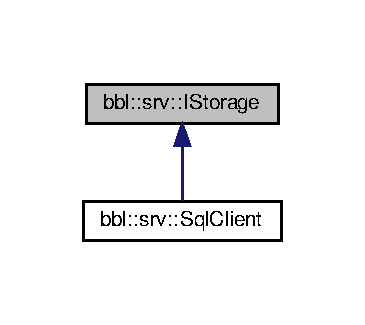
\includegraphics[width=175pt]{classbbl_1_1srv_1_1_i_storage__inherit__graph}
\end{center}
\end{figure}
\subsection*{Public Member Functions}
\begin{DoxyCompactItemize}
\item 
\mbox{\Hypertarget{classbbl_1_1srv_1_1_i_storage_ae573fbede5dc6e839878d105d5ed9c7f}\label{classbbl_1_1srv_1_1_i_storage_ae573fbede5dc6e839878d105d5ed9c7f}} 
virtual void {\bfseries register\+User} (const std\+::string \&username, const std\+::string \&password) const =0
\item 
\mbox{\Hypertarget{classbbl_1_1srv_1_1_i_storage_a25f5dd59922a95e81cce022af1446f55}\label{classbbl_1_1srv_1_1_i_storage_a25f5dd59922a95e81cce022af1446f55}} 
virtual void {\bfseries login\+User} (const std\+::string \&username, const std\+::string \&password) const =0
\item 
\mbox{\Hypertarget{classbbl_1_1srv_1_1_i_storage_afdca8afce2681f2a6a7388962bb578f9}\label{classbbl_1_1srv_1_1_i_storage_afdca8afce2681f2a6a7388962bb578f9}} 
virtual std\+::vector$<$ std\+::string $>$ {\bfseries get\+Contacts} (const std\+::string \&username) const =0
\item 
\mbox{\Hypertarget{classbbl_1_1srv_1_1_i_storage_a2e3541635272914292fe5e70dd5d071b}\label{classbbl_1_1srv_1_1_i_storage_a2e3541635272914292fe5e70dd5d071b}} 
virtual std\+::vector$<$ std\+::string $>$ {\bfseries get\+Requests} (const std\+::string \&username) const =0
\item 
\mbox{\Hypertarget{classbbl_1_1srv_1_1_i_storage_aff2a9b83a9076eba98b837821d8593ab}\label{classbbl_1_1srv_1_1_i_storage_aff2a9b83a9076eba98b837821d8593ab}} 
virtual void {\bfseries add\+Request} (const std\+::string \&owner, const std\+::string \&contact) const =0
\item 
\mbox{\Hypertarget{classbbl_1_1srv_1_1_i_storage_a2ff99f698e40d39a298746d53602e990}\label{classbbl_1_1srv_1_1_i_storage_a2ff99f698e40d39a298746d53602e990}} 
virtual void {\bfseries accept\+Request} (const std\+::string \&owner, const std\+::string \&contact) const =0
\item 
\mbox{\Hypertarget{classbbl_1_1srv_1_1_i_storage_ac1d86f612146cfc3188fa06b4ea767ea}\label{classbbl_1_1srv_1_1_i_storage_ac1d86f612146cfc3188fa06b4ea767ea}} 
virtual void {\bfseries set\+Udp\+Parameters} (const std\+::string \&owner, const std\+::string \&ipv4, const std\+::string \&port) const =0
\item 
\mbox{\Hypertarget{classbbl_1_1srv_1_1_i_storage_acc8ca98c6bb8059c5bfeef056e5a146b}\label{classbbl_1_1srv_1_1_i_storage_acc8ca98c6bb8059c5bfeef056e5a146b}} 
virtual std\+::array$<$ std\+::string, 2 $>$ {\bfseries get\+Udp\+Parameters} (const std\+::string \&owner, const std\+::string \&me) const =0
\end{DoxyCompactItemize}


The documentation for this class was generated from the following file\+:\begin{DoxyCompactItemize}
\item 
Server/include/\+Storage/I\+Storage.\+hpp\end{DoxyCompactItemize}

\hypertarget{class_i_stream}{}\section{I\+Stream Class Reference}
\label{class_i_stream}\index{I\+Stream@{I\+Stream}}


Inheritance diagram for I\+Stream\+:
\nopagebreak
\begin{figure}[H]
\begin{center}
\leavevmode
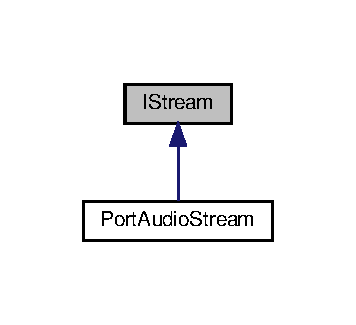
\includegraphics[width=171pt]{class_i_stream__inherit__graph}
\end{center}
\end{figure}
\subsection*{Public Member Functions}
\begin{DoxyCompactItemize}
\item 
\mbox{\Hypertarget{class_i_stream_a844cd2b5207b323ba158d765d4441199}\label{class_i_stream_a844cd2b5207b323ba158d765d4441199}} 
virtual void {\bfseries Open\+Stream\+Recorder} ()=0
\item 
\mbox{\Hypertarget{class_i_stream_a71920441111ee52b6269e77adb455f51}\label{class_i_stream_a71920441111ee52b6269e77adb455f51}} 
virtual void {\bfseries Open\+Stream\+Player} ()=0
\item 
\mbox{\Hypertarget{class_i_stream_a3b8cf2e054144598b50041174a3be595}\label{class_i_stream_a3b8cf2e054144598b50041174a3be595}} 
virtual void {\bfseries Start\+Stream} ()=0
\end{DoxyCompactItemize}


The documentation for this class was generated from the following file\+:\begin{DoxyCompactItemize}
\item 
Client/include/\+Audio/I\+Stream.\+hpp\end{DoxyCompactItemize}

\hypertarget{classbbl_1_1cli_1_1_i_tcp_client}{}\section{bbl\+:\+:cli\+:\+:I\+Tcp\+Client Class Reference}
\label{classbbl_1_1cli_1_1_i_tcp_client}\index{bbl\+::cli\+::\+I\+Tcp\+Client@{bbl\+::cli\+::\+I\+Tcp\+Client}}


Inheritance diagram for bbl\+:\+:cli\+:\+:I\+Tcp\+Client\+:
\nopagebreak
\begin{figure}[H]
\begin{center}
\leavevmode
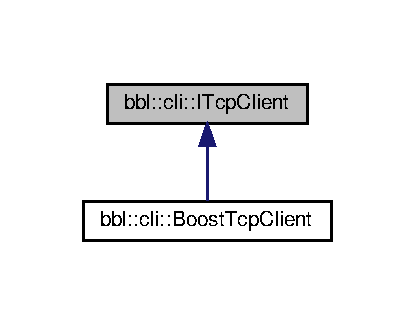
\includegraphics[width=199pt]{classbbl_1_1cli_1_1_i_tcp_client__inherit__graph}
\end{center}
\end{figure}
\subsection*{Public Member Functions}
\begin{DoxyCompactItemize}
\item 
\mbox{\Hypertarget{classbbl_1_1cli_1_1_i_tcp_client_a46cc16cc1a32f452aeafa26aae911748}\label{classbbl_1_1cli_1_1_i_tcp_client_a46cc16cc1a32f452aeafa26aae911748}} 
virtual void {\bfseries send} (const std\+::string \&data)=0
\item 
\mbox{\Hypertarget{classbbl_1_1cli_1_1_i_tcp_client_a3c849d6c7f7800d4c8fdacef36800ab6}\label{classbbl_1_1cli_1_1_i_tcp_client_a3c849d6c7f7800d4c8fdacef36800ab6}} 
virtual std\+::string {\bfseries recv} ()=0
\end{DoxyCompactItemize}


The documentation for this class was generated from the following file\+:\begin{DoxyCompactItemize}
\item 
Client/include/\+Network/I\+Tcp\+Client.\+hpp\end{DoxyCompactItemize}

\hypertarget{classbbl_1_1cli_1_1_i_udp_client}{}\section{bbl\+:\+:cli\+:\+:I\+Udp\+Client Class Reference}
\label{classbbl_1_1cli_1_1_i_udp_client}\index{bbl\+::cli\+::\+I\+Udp\+Client@{bbl\+::cli\+::\+I\+Udp\+Client}}


Inheritance diagram for bbl\+:\+:cli\+:\+:I\+Udp\+Client\+:
\nopagebreak
\begin{figure}[H]
\begin{center}
\leavevmode
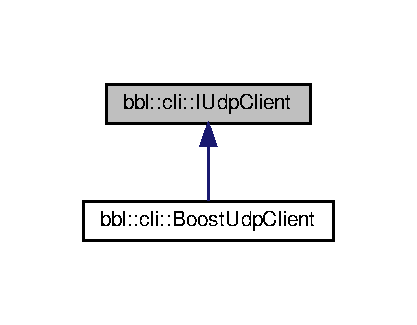
\includegraphics[width=200pt]{classbbl_1_1cli_1_1_i_udp_client__inherit__graph}
\end{center}
\end{figure}
\subsection*{Public Member Functions}
\begin{DoxyCompactItemize}
\item 
\mbox{\Hypertarget{classbbl_1_1cli_1_1_i_udp_client_a363210532b30e3d9d3fb8027afe1966d}\label{classbbl_1_1cli_1_1_i_udp_client_a363210532b30e3d9d3fb8027afe1966d}} 
virtual void {\bfseries send} (const \hyperlink{classbbl_1_1cli_1_1_packet}{Packet} \&packet)=0
\item 
\mbox{\Hypertarget{classbbl_1_1cli_1_1_i_udp_client_a05160445368a5b5d383071e5f5bdd0ce}\label{classbbl_1_1cli_1_1_i_udp_client_a05160445368a5b5d383071e5f5bdd0ce}} 
virtual \hyperlink{classbbl_1_1cli_1_1_packet}{Packet} {\bfseries recv} ()=0
\item 
\mbox{\Hypertarget{classbbl_1_1cli_1_1_i_udp_client_a4b4427523117a063cae8044111326887}\label{classbbl_1_1cli_1_1_i_udp_client_a4b4427523117a063cae8044111326887}} 
virtual unsigned short {\bfseries get\+Port} () const =0
\item 
\mbox{\Hypertarget{classbbl_1_1cli_1_1_i_udp_client_a3106102e589e98e357a3a7d555f21813}\label{classbbl_1_1cli_1_1_i_udp_client_a3106102e589e98e357a3a7d555f21813}} 
virtual void {\bfseries close} ()=0
\end{DoxyCompactItemize}


The documentation for this class was generated from the following file\+:\begin{DoxyCompactItemize}
\item 
Client/include/\+Network/I\+Udp\+Client.\+hpp\end{DoxyCompactItemize}

\hypertarget{classbbl_1_1cli_1_1graphics_1_1_i_window}{}\section{bbl\+:\+:cli\+:\+:graphics\+:\+:I\+Window Class Reference}
\label{classbbl_1_1cli_1_1graphics_1_1_i_window}\index{bbl\+::cli\+::graphics\+::\+I\+Window@{bbl\+::cli\+::graphics\+::\+I\+Window}}


Inheritance diagram for bbl\+:\+:cli\+:\+:graphics\+:\+:I\+Window\+:
\nopagebreak
\begin{figure}[H]
\begin{center}
\leavevmode
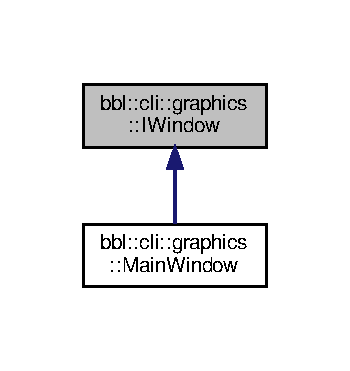
\includegraphics[width=168pt]{classbbl_1_1cli_1_1graphics_1_1_i_window__inherit__graph}
\end{center}
\end{figure}
\subsection*{Public Member Functions}
\begin{DoxyCompactItemize}
\item 
\mbox{\Hypertarget{classbbl_1_1cli_1_1graphics_1_1_i_window_a56dd4f3ebede9e43ca66d119a0a93d52}\label{classbbl_1_1cli_1_1graphics_1_1_i_window_a56dd4f3ebede9e43ca66d119a0a93d52}} 
virtual void {\bfseries login} (const Q\+String \&login, const Q\+String \&password)=0
\item 
\mbox{\Hypertarget{classbbl_1_1cli_1_1graphics_1_1_i_window_ac1accfd03df96f03c4d256ffa2e6cbd6}\label{classbbl_1_1cli_1_1graphics_1_1_i_window_ac1accfd03df96f03c4d256ffa2e6cbd6}} 
virtual void {\bfseries signup} (const Q\+String \&login, const Q\+String \&password)=0
\item 
\mbox{\Hypertarget{classbbl_1_1cli_1_1graphics_1_1_i_window_aff4654f7f04ae6154c47992f6ab26ae6}\label{classbbl_1_1cli_1_1graphics_1_1_i_window_aff4654f7f04ae6154c47992f6ab26ae6}} 
virtual \hyperlink{classbbl_1_1cli_1_1_client}{Client} \& {\bfseries get\+Client} ()=0
\end{DoxyCompactItemize}


The documentation for this class was generated from the following file\+:\begin{DoxyCompactItemize}
\item 
Client/include/\+Graphic/I\+Window.\+hpp\end{DoxyCompactItemize}

\hypertarget{classbbl_1_1srv_1_1_login_command}{}\section{bbl\+:\+:srv\+:\+:Login\+Command Class Reference}
\label{classbbl_1_1srv_1_1_login_command}\index{bbl\+::srv\+::\+Login\+Command@{bbl\+::srv\+::\+Login\+Command}}
\subsection*{Static Public Member Functions}
\begin{DoxyCompactItemize}
\item 
\mbox{\Hypertarget{classbbl_1_1srv_1_1_login_command_a8ea3bc8b736cab226924094181d83bd0}\label{classbbl_1_1srv_1_1_login_command_a8ea3bc8b736cab226924094181d83bd0}} 
static void {\bfseries run} (std\+::vector$<$ \hyperlink{classbbl_1_1srv_1_1_user}{User} $\ast$$>$ \+\_\+clients, \hyperlink{classbbl_1_1srv_1_1_user}{User} $\ast$current, \hyperlink{classbbl_1_1srv_1_1_i_storage}{I\+Storage} $\ast$db, const std\+::vector$<$ std\+::string $>$ \&av)
\end{DoxyCompactItemize}


The documentation for this class was generated from the following file\+:\begin{DoxyCompactItemize}
\item 
Server/include/\+Core/Login\+Command.\+hpp\end{DoxyCompactItemize}

\hypertarget{classbbl_1_1srv_1_1_logout_command}{}\section{bbl\+:\+:srv\+:\+:Logout\+Command Class Reference}
\label{classbbl_1_1srv_1_1_logout_command}\index{bbl\+::srv\+::\+Logout\+Command@{bbl\+::srv\+::\+Logout\+Command}}
\subsection*{Static Public Member Functions}
\begin{DoxyCompactItemize}
\item 
\mbox{\Hypertarget{classbbl_1_1srv_1_1_logout_command_a2c51ad737f53fa197d082cefba3c3509}\label{classbbl_1_1srv_1_1_logout_command_a2c51ad737f53fa197d082cefba3c3509}} 
static void {\bfseries run} (std\+::vector$<$ \hyperlink{classbbl_1_1srv_1_1_user}{User} $\ast$$>$ \+\_\+clients, \hyperlink{classbbl_1_1srv_1_1_user}{User} $\ast$current, \hyperlink{classbbl_1_1srv_1_1_i_storage}{I\+Storage} $\ast$db, const std\+::vector$<$ std\+::string $>$ \&av)
\end{DoxyCompactItemize}


The documentation for this class was generated from the following file\+:\begin{DoxyCompactItemize}
\item 
Server/include/\+Core/Logout\+Command.\+hpp\end{DoxyCompactItemize}

\hypertarget{classbbl_1_1cli_1_1graphics_1_1_main_window}{}\section{bbl\+:\+:cli\+:\+:graphics\+:\+:Main\+Window Class Reference}
\label{classbbl_1_1cli_1_1graphics_1_1_main_window}\index{bbl\+::cli\+::graphics\+::\+Main\+Window@{bbl\+::cli\+::graphics\+::\+Main\+Window}}


Inheritance diagram for bbl\+:\+:cli\+:\+:graphics\+:\+:Main\+Window\+:
\nopagebreak
\begin{figure}[H]
\begin{center}
\leavevmode
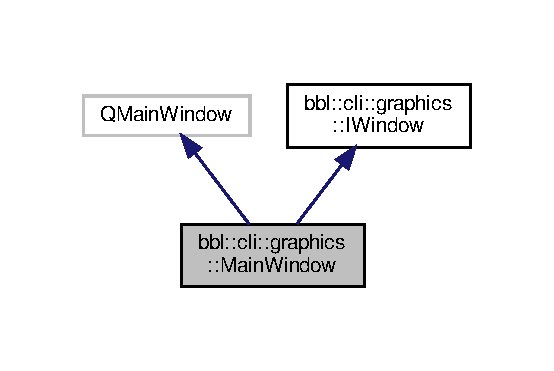
\includegraphics[width=266pt]{classbbl_1_1cli_1_1graphics_1_1_main_window__inherit__graph}
\end{center}
\end{figure}


Collaboration diagram for bbl\+:\+:cli\+:\+:graphics\+:\+:Main\+Window\+:
\nopagebreak
\begin{figure}[H]
\begin{center}
\leavevmode
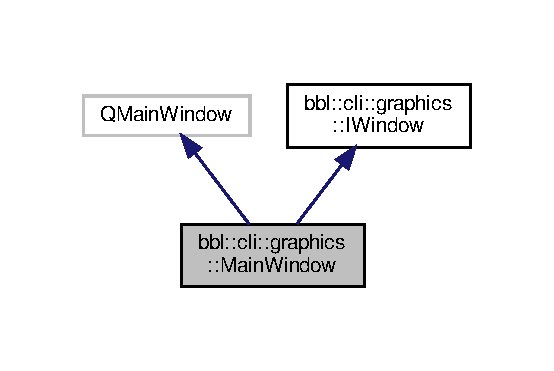
\includegraphics[width=266pt]{classbbl_1_1cli_1_1graphics_1_1_main_window__coll__graph}
\end{center}
\end{figure}
\subsection*{Public Slots}
\begin{DoxyCompactItemize}
\item 
\mbox{\Hypertarget{classbbl_1_1cli_1_1graphics_1_1_main_window_ae857b62241e491a5555ed489014dcf1f}\label{classbbl_1_1cli_1_1graphics_1_1_main_window_ae857b62241e491a5555ed489014dcf1f}} 
void {\bfseries go\+Signup} ()
\item 
\mbox{\Hypertarget{classbbl_1_1cli_1_1graphics_1_1_main_window_af020576ab1d1e0e7050f2bf73e018188}\label{classbbl_1_1cli_1_1graphics_1_1_main_window_af020576ab1d1e0e7050f2bf73e018188}} 
void {\bfseries go\+Signin} ()
\end{DoxyCompactItemize}
\subsection*{Public Member Functions}
\begin{DoxyCompactItemize}
\item 
\mbox{\Hypertarget{classbbl_1_1cli_1_1graphics_1_1_main_window_adc89b3344ef0a716d5301e94ae61d784}\label{classbbl_1_1cli_1_1graphics_1_1_main_window_adc89b3344ef0a716d5301e94ae61d784}} 
void {\bfseries login} (const Q\+String \&login, const Q\+String \&password)
\item 
\mbox{\Hypertarget{classbbl_1_1cli_1_1graphics_1_1_main_window_adc7a86fda96a758fd16a6cc86ab8ce2c}\label{classbbl_1_1cli_1_1graphics_1_1_main_window_adc7a86fda96a758fd16a6cc86ab8ce2c}} 
void {\bfseries signup} (const Q\+String \&login, const Q\+String \&password)
\item 
\mbox{\Hypertarget{classbbl_1_1cli_1_1graphics_1_1_main_window_ac247f6f688a0793541a517aa689b43cc}\label{classbbl_1_1cli_1_1graphics_1_1_main_window_ac247f6f688a0793541a517aa689b43cc}} 
\hyperlink{classbbl_1_1cli_1_1_client}{Client} \& {\bfseries get\+Client} ()
\item 
\mbox{\Hypertarget{classbbl_1_1cli_1_1graphics_1_1_main_window_a39f535d7e99763b58ee9415d95f412fa}\label{classbbl_1_1cli_1_1graphics_1_1_main_window_a39f535d7e99763b58ee9415d95f412fa}} 
void {\bfseries go\+Contacts} ()
\item 
\mbox{\Hypertarget{classbbl_1_1cli_1_1graphics_1_1_main_window_a4e20a4a065fbb0e4d3532a45a0a91425}\label{classbbl_1_1cli_1_1graphics_1_1_main_window_a4e20a4a065fbb0e4d3532a45a0a91425}} 
void {\bfseries close\+Event} (Q\+Close\+Event $\ast$event)
\end{DoxyCompactItemize}


The documentation for this class was generated from the following files\+:\begin{DoxyCompactItemize}
\item 
Client/include/\+Graphic/Main\+Window.\+hpp\item 
Client/src/\+Graphic/Main\+Window.\+cpp\end{DoxyCompactItemize}

\hypertarget{classbbl_1_1srv_1_1_network_manager}{}\section{bbl\+:\+:srv\+:\+:Network\+Manager Class Reference}
\label{classbbl_1_1srv_1_1_network_manager}\index{bbl\+::srv\+::\+Network\+Manager@{bbl\+::srv\+::\+Network\+Manager}}
\subsection*{Public Member Functions}
\begin{DoxyCompactItemize}
\item 
\mbox{\Hypertarget{classbbl_1_1srv_1_1_network_manager_a0eef19acc78e74b6d05e26cce6985c84}\label{classbbl_1_1srv_1_1_network_manager_a0eef19acc78e74b6d05e26cce6985c84}} 
{\bfseries Network\+Manager} (\hyperlink{classbbl_1_1srv_1_1_i_storage}{I\+Storage} $\ast$database)
\item 
\mbox{\Hypertarget{classbbl_1_1srv_1_1_network_manager_a1cf6832dd4e67937f407e230db86bfa4}\label{classbbl_1_1srv_1_1_network_manager_a1cf6832dd4e67937f407e230db86bfa4}} 
void {\bfseries new\+Client} (\hyperlink{classbbl_1_1srv_1_1_i_network_client}{I\+Network\+Client} $\ast$client)
\item 
\mbox{\Hypertarget{classbbl_1_1srv_1_1_network_manager_a62b74532f1ffd1882460ac8c4dcc56ba}\label{classbbl_1_1srv_1_1_network_manager_a62b74532f1ffd1882460ac8c4dcc56ba}} 
void {\bfseries remove\+Client} (\hyperlink{classbbl_1_1srv_1_1_i_network_client}{I\+Network\+Client} $\ast$client)
\item 
\mbox{\Hypertarget{classbbl_1_1srv_1_1_network_manager_a77a7757450eef7c970673e615ea14e1b}\label{classbbl_1_1srv_1_1_network_manager_a77a7757450eef7c970673e615ea14e1b}} 
void {\bfseries recv\+Data} (\hyperlink{classbbl_1_1srv_1_1_i_network_client}{I\+Network\+Client} $\ast$client, const std\+::string \&data)
\item 
\mbox{\Hypertarget{classbbl_1_1srv_1_1_network_manager_a338ea0d2cc3a1db5f72bc1f1e778e5f3}\label{classbbl_1_1srv_1_1_network_manager_a338ea0d2cc3a1db5f72bc1f1e778e5f3}} 
{\bfseries Network\+Manager} (const \hyperlink{classbbl_1_1srv_1_1_network_manager}{Network\+Manager} \&)=delete
\item 
\mbox{\Hypertarget{classbbl_1_1srv_1_1_network_manager_a33772329a1bcbe58e560ead6ac8677d4}\label{classbbl_1_1srv_1_1_network_manager_a33772329a1bcbe58e560ead6ac8677d4}} 
\hyperlink{classbbl_1_1srv_1_1_network_manager}{Network\+Manager} \& {\bfseries operator=} (const \hyperlink{classbbl_1_1srv_1_1_network_manager}{Network\+Manager} \&)=delete
\end{DoxyCompactItemize}


The documentation for this class was generated from the following files\+:\begin{DoxyCompactItemize}
\item 
Server/include/\+Network/Network\+Manager.\+hpp\item 
Server/src/\+Network/Network\+Manager.\+cpp\end{DoxyCompactItemize}

\hypertarget{classbbl_1_1cli_1_1_packet}{}\section{bbl\+:\+:cli\+:\+:Packet Class Reference}
\label{classbbl_1_1cli_1_1_packet}\index{bbl\+::cli\+::\+Packet@{bbl\+::cli\+::\+Packet}}
\subsection*{Public Member Functions}
\begin{DoxyCompactItemize}
\item 
\mbox{\Hypertarget{classbbl_1_1cli_1_1_packet_a76b04619266ab2ae7fd7c14c50a1c5f7}\label{classbbl_1_1cli_1_1_packet_a76b04619266ab2ae7fd7c14c50a1c5f7}} 
{\bfseries Packet} (const std\+::vector$<$ unsigned char $>$ \&data)
\item 
\mbox{\Hypertarget{classbbl_1_1cli_1_1_packet_a84b84b6bbf21b76fc5769be81b4a8395}\label{classbbl_1_1cli_1_1_packet_a84b84b6bbf21b76fc5769be81b4a8395}} 
{\bfseries Packet} (const unsigned char $\ast$data, std\+::size\+\_\+t length)
\item 
\mbox{\Hypertarget{classbbl_1_1cli_1_1_packet_a81860a16fe26b2d3d362fba4668264bf}\label{classbbl_1_1cli_1_1_packet_a81860a16fe26b2d3d362fba4668264bf}} 
{\bfseries Packet} (const \hyperlink{classbbl_1_1cli_1_1_packet}{Packet} \&copy)
\item 
\mbox{\Hypertarget{classbbl_1_1cli_1_1_packet_a5cc278dcde53bfcb8cd77c3704880bae}\label{classbbl_1_1cli_1_1_packet_a5cc278dcde53bfcb8cd77c3704880bae}} 
\hyperlink{classbbl_1_1cli_1_1_packet}{Packet} \& {\bfseries operator=} (const \hyperlink{classbbl_1_1cli_1_1_packet}{Packet} \&copy)
\item 
\mbox{\Hypertarget{classbbl_1_1cli_1_1_packet_a82d910e8390eeb56c79c8610daa789b7}\label{classbbl_1_1cli_1_1_packet_a82d910e8390eeb56c79c8610daa789b7}} 
void {\bfseries append} (const std\+::vector$<$ unsigned char $>$ \&data)
\item 
\mbox{\Hypertarget{classbbl_1_1cli_1_1_packet_a8a6375187b78746db5145088c1f4a9bc}\label{classbbl_1_1cli_1_1_packet_a8a6375187b78746db5145088c1f4a9bc}} 
void {\bfseries append} (const unsigned char $\ast$data, std\+::size\+\_\+t length)
\item 
\mbox{\Hypertarget{classbbl_1_1cli_1_1_packet_aebfe64af8bdfbc3afce09ce0f33d64ff}\label{classbbl_1_1cli_1_1_packet_aebfe64af8bdfbc3afce09ce0f33d64ff}} 
const std\+::vector$<$ unsigned char $>$ \& {\bfseries get\+Data} () const
\end{DoxyCompactItemize}


The documentation for this class was generated from the following files\+:\begin{DoxyCompactItemize}
\item 
Client/include/\+Network/Packet.\+hpp\item 
Client/src/\+Network/Packet.\+cpp\end{DoxyCompactItemize}

\hypertarget{class_port_audio_input}{}\section{Port\+Audio\+Input Class Reference}
\label{class_port_audio_input}\index{Port\+Audio\+Input@{Port\+Audio\+Input}}


Inheritance diagram for Port\+Audio\+Input\+:
\nopagebreak
\begin{figure}[H]
\begin{center}
\leavevmode
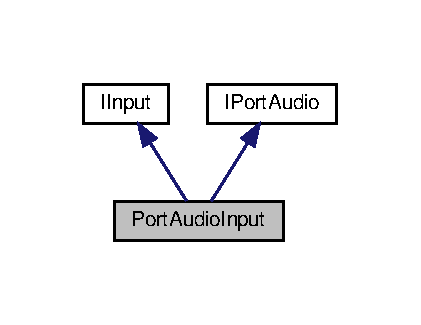
\includegraphics[width=202pt]{class_port_audio_input__inherit__graph}
\end{center}
\end{figure}


Collaboration diagram for Port\+Audio\+Input\+:
\nopagebreak
\begin{figure}[H]
\begin{center}
\leavevmode
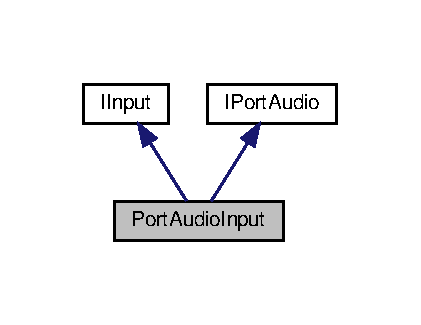
\includegraphics[width=202pt]{class_port_audio_input__coll__graph}
\end{center}
\end{figure}
\subsection*{Public Member Functions}
\begin{DoxyCompactItemize}
\item 
\mbox{\Hypertarget{class_port_audio_input_a178d6babb3762d1e4d1d61bd41c976ae}\label{class_port_audio_input_a178d6babb3762d1e4d1d61bd41c976ae}} 
{\bfseries Port\+Audio\+Input} (int i)
\item 
\mbox{\Hypertarget{class_port_audio_input_a8bfa09888eae1a4ba66b834ca60889f7}\label{class_port_audio_input_a8bfa09888eae1a4ba66b834ca60889f7}} 
Pa\+Stream\+Parameters {\bfseries get\+Parameters} () const
\item 
\mbox{\Hypertarget{class_port_audio_input_a137f30910ee1a1c264ff066dce1bf821}\label{class_port_audio_input_a137f30910ee1a1c264ff066dce1bf821}} 
void {\bfseries set\+Parameters} (const Pa\+Stream\+Parameters get\+Input\+Parameters)
\end{DoxyCompactItemize}


The documentation for this class was generated from the following files\+:\begin{DoxyCompactItemize}
\item 
Client/include/\+Audio/Port\+Audio\+Input.\+hpp\item 
Client/src/\+Audio/Port\+Audio\+Input.\+cpp\end{DoxyCompactItemize}

\hypertarget{class_port_audio_output}{}\section{Port\+Audio\+Output Class Reference}
\label{class_port_audio_output}\index{Port\+Audio\+Output@{Port\+Audio\+Output}}


Inheritance diagram for Port\+Audio\+Output\+:
\nopagebreak
\begin{figure}[H]
\begin{center}
\leavevmode
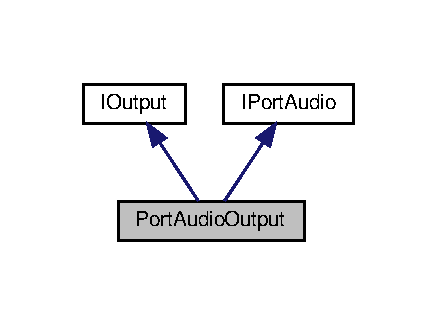
\includegraphics[width=210pt]{class_port_audio_output__inherit__graph}
\end{center}
\end{figure}


Collaboration diagram for Port\+Audio\+Output\+:
\nopagebreak
\begin{figure}[H]
\begin{center}
\leavevmode
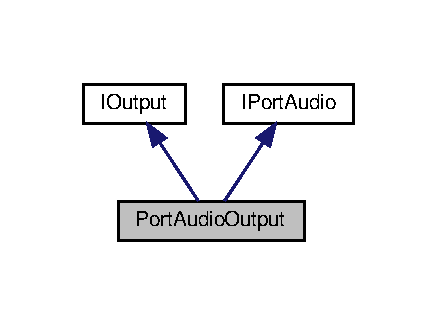
\includegraphics[width=210pt]{class_port_audio_output__coll__graph}
\end{center}
\end{figure}
\subsection*{Public Member Functions}
\begin{DoxyCompactItemize}
\item 
\mbox{\Hypertarget{class_port_audio_output_ab50175e3867e2d907ce801ae12534391}\label{class_port_audio_output_ab50175e3867e2d907ce801ae12534391}} 
{\bfseries Port\+Audio\+Output} (int i)
\item 
\mbox{\Hypertarget{class_port_audio_output_a4eea0854943fb1bc254bbad6147147da}\label{class_port_audio_output_a4eea0854943fb1bc254bbad6147147da}} 
Pa\+Stream\+Parameters {\bfseries get\+Parameters} () const
\item 
\mbox{\Hypertarget{class_port_audio_output_a4feee44264636b7b32e502d1e8638778}\label{class_port_audio_output_a4feee44264636b7b32e502d1e8638778}} 
void {\bfseries set\+Parameters} (const Pa\+Stream\+Parameters get\+Output\+Parameters)
\end{DoxyCompactItemize}


The documentation for this class was generated from the following files\+:\begin{DoxyCompactItemize}
\item 
Client/include/\+Audio/Port\+Audio\+Output.\+hpp\item 
Client/src/\+Audio/Port\+Audio\+Output.\+cpp\end{DoxyCompactItemize}

\hypertarget{class_port_audio_stream}{}\section{Port\+Audio\+Stream Class Reference}
\label{class_port_audio_stream}\index{Port\+Audio\+Stream@{Port\+Audio\+Stream}}


Inheritance diagram for Port\+Audio\+Stream\+:
\nopagebreak
\begin{figure}[H]
\begin{center}
\leavevmode
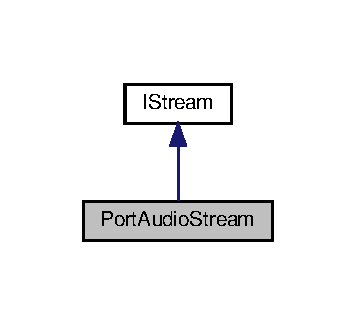
\includegraphics[width=171pt]{class_port_audio_stream__inherit__graph}
\end{center}
\end{figure}


Collaboration diagram for Port\+Audio\+Stream\+:
\nopagebreak
\begin{figure}[H]
\begin{center}
\leavevmode
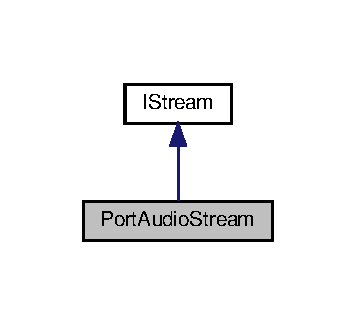
\includegraphics[width=171pt]{class_port_audio_stream__coll__graph}
\end{center}
\end{figure}
\subsection*{Public Member Functions}
\begin{DoxyCompactItemize}
\item 
\mbox{\Hypertarget{class_port_audio_stream_adca8e4d379d44412dea3e92143270e26}\label{class_port_audio_stream_adca8e4d379d44412dea3e92143270e26}} 
{\bfseries Port\+Audio\+Stream} (Pa\+Stream\+Parameters input, Pa\+Stream\+Parameters output, \hyperlink{class_audio_data}{Audio\+Data} $\ast$data)
\item 
\mbox{\Hypertarget{class_port_audio_stream_ab750710cae4d8e1c0f1bb771a73bedfe}\label{class_port_audio_stream_ab750710cae4d8e1c0f1bb771a73bedfe}} 
void {\bfseries Open\+Stream\+Recorder} ()
\item 
\mbox{\Hypertarget{class_port_audio_stream_ab6e03287c72e34984d05510a61797e7a}\label{class_port_audio_stream_ab6e03287c72e34984d05510a61797e7a}} 
void {\bfseries Open\+Stream\+Player} ()
\item 
\mbox{\Hypertarget{class_port_audio_stream_aa2fa5f227ea2770fe9ce56d01703097c}\label{class_port_audio_stream_aa2fa5f227ea2770fe9ce56d01703097c}} 
void {\bfseries Start\+Stream} ()
\end{DoxyCompactItemize}


The documentation for this class was generated from the following files\+:\begin{DoxyCompactItemize}
\item 
Client/include/\+Audio/Port\+Audio\+Stream.\+hpp\item 
Client/src/\+Audio/Port\+Audio\+Stream.\+cpp\end{DoxyCompactItemize}

\hypertarget{classbbl_1_1srv_1_1_register_command}{}\section{bbl\+:\+:srv\+:\+:Register\+Command Class Reference}
\label{classbbl_1_1srv_1_1_register_command}\index{bbl\+::srv\+::\+Register\+Command@{bbl\+::srv\+::\+Register\+Command}}
\subsection*{Static Public Member Functions}
\begin{DoxyCompactItemize}
\item 
\mbox{\Hypertarget{classbbl_1_1srv_1_1_register_command_a6ce7258c3ba03021be83931e1df9b6ae}\label{classbbl_1_1srv_1_1_register_command_a6ce7258c3ba03021be83931e1df9b6ae}} 
static void {\bfseries run} (std\+::vector$<$ \hyperlink{classbbl_1_1srv_1_1_user}{User} $\ast$$>$ \+\_\+clients, \hyperlink{classbbl_1_1srv_1_1_user}{User} $\ast$current, \hyperlink{classbbl_1_1srv_1_1_i_storage}{I\+Storage} $\ast$db, const std\+::vector$<$ std\+::string $>$ \&av)
\end{DoxyCompactItemize}


The documentation for this class was generated from the following file\+:\begin{DoxyCompactItemize}
\item 
Server/include/\+Core/Register\+Command.\+hpp\end{DoxyCompactItemize}

\hypertarget{classbbl_1_1srv_1_1_set_udp_command}{}\section{bbl\+:\+:srv\+:\+:Set\+Udp\+Command Class Reference}
\label{classbbl_1_1srv_1_1_set_udp_command}\index{bbl\+::srv\+::\+Set\+Udp\+Command@{bbl\+::srv\+::\+Set\+Udp\+Command}}
\subsection*{Static Public Member Functions}
\begin{DoxyCompactItemize}
\item 
\mbox{\Hypertarget{classbbl_1_1srv_1_1_set_udp_command_aad8d38f9c3f1740805c20ee5547221ee}\label{classbbl_1_1srv_1_1_set_udp_command_aad8d38f9c3f1740805c20ee5547221ee}} 
static void {\bfseries run} (std\+::vector$<$ \hyperlink{classbbl_1_1srv_1_1_user}{User} $\ast$$>$ \+\_\+clients, \hyperlink{classbbl_1_1srv_1_1_user}{User} $\ast$current, \hyperlink{classbbl_1_1srv_1_1_i_storage}{I\+Storage} $\ast$db, const std\+::vector$<$ std\+::string $>$ \&av)
\end{DoxyCompactItemize}


The documentation for this class was generated from the following file\+:\begin{DoxyCompactItemize}
\item 
Server/include/\+Core/Set\+Udp\+Command.\+hpp\end{DoxyCompactItemize}

\hypertarget{classbbl_1_1cli_1_1graphics_1_1_signin_form}{}\section{bbl\+:\+:cli\+:\+:graphics\+:\+:Signin\+Form Class Reference}
\label{classbbl_1_1cli_1_1graphics_1_1_signin_form}\index{bbl\+::cli\+::graphics\+::\+Signin\+Form@{bbl\+::cli\+::graphics\+::\+Signin\+Form}}


Inheritance diagram for bbl\+:\+:cli\+:\+:graphics\+:\+:Signin\+Form\+:
\nopagebreak
\begin{figure}[H]
\begin{center}
\leavevmode
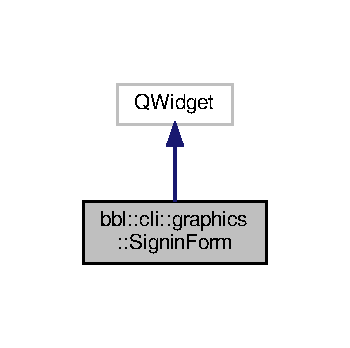
\includegraphics[width=168pt]{classbbl_1_1cli_1_1graphics_1_1_signin_form__inherit__graph}
\end{center}
\end{figure}


Collaboration diagram for bbl\+:\+:cli\+:\+:graphics\+:\+:Signin\+Form\+:
\nopagebreak
\begin{figure}[H]
\begin{center}
\leavevmode
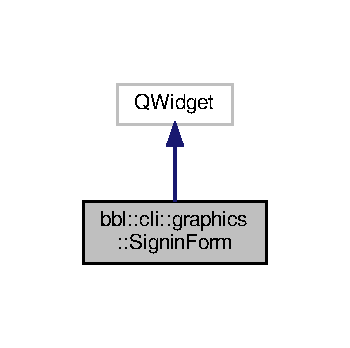
\includegraphics[width=168pt]{classbbl_1_1cli_1_1graphics_1_1_signin_form__coll__graph}
\end{center}
\end{figure}
\subsection*{Public Slots}
\begin{DoxyCompactItemize}
\item 
\mbox{\Hypertarget{classbbl_1_1cli_1_1graphics_1_1_signin_form_ac239f8fd91cc0b8f58aba3a377cad960}\label{classbbl_1_1cli_1_1graphics_1_1_signin_form_ac239f8fd91cc0b8f58aba3a377cad960}} 
void {\bfseries login} ()
\end{DoxyCompactItemize}
\subsection*{Public Member Functions}
\begin{DoxyCompactItemize}
\item 
\mbox{\Hypertarget{classbbl_1_1cli_1_1graphics_1_1_signin_form_ad24e01fe8f02d700e49e15b67794aff0}\label{classbbl_1_1cli_1_1graphics_1_1_signin_form_ad24e01fe8f02d700e49e15b67794aff0}} 
{\bfseries Signin\+Form} (Q\+Main\+Window $\ast$parent)
\end{DoxyCompactItemize}


The documentation for this class was generated from the following files\+:\begin{DoxyCompactItemize}
\item 
Client/include/\+Graphic/Signin\+Form.\+hpp\item 
Client/src/\+Graphic/Signin\+Form.\+cpp\end{DoxyCompactItemize}

\hypertarget{classbbl_1_1cli_1_1graphics_1_1_signup_form}{}\section{bbl\+:\+:cli\+:\+:graphics\+:\+:Signup\+Form Class Reference}
\label{classbbl_1_1cli_1_1graphics_1_1_signup_form}\index{bbl\+::cli\+::graphics\+::\+Signup\+Form@{bbl\+::cli\+::graphics\+::\+Signup\+Form}}


Inheritance diagram for bbl\+:\+:cli\+:\+:graphics\+:\+:Signup\+Form\+:
\nopagebreak
\begin{figure}[H]
\begin{center}
\leavevmode
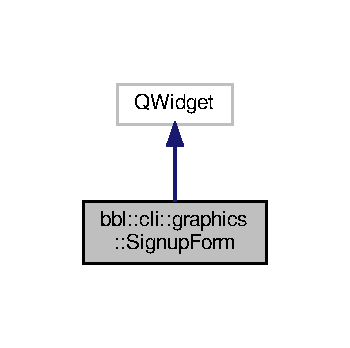
\includegraphics[width=168pt]{classbbl_1_1cli_1_1graphics_1_1_signup_form__inherit__graph}
\end{center}
\end{figure}


Collaboration diagram for bbl\+:\+:cli\+:\+:graphics\+:\+:Signup\+Form\+:
\nopagebreak
\begin{figure}[H]
\begin{center}
\leavevmode
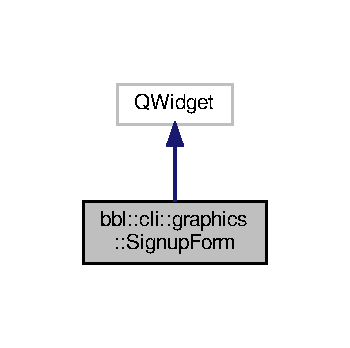
\includegraphics[width=168pt]{classbbl_1_1cli_1_1graphics_1_1_signup_form__coll__graph}
\end{center}
\end{figure}
\subsection*{Public Slots}
\begin{DoxyCompactItemize}
\item 
\mbox{\Hypertarget{classbbl_1_1cli_1_1graphics_1_1_signup_form_a2d0783bca931ef03fb674226cd6d75f4}\label{classbbl_1_1cli_1_1graphics_1_1_signup_form_a2d0783bca931ef03fb674226cd6d75f4}} 
void {\bfseries on\+Password\+Edit} (const Q\+String \&text)
\item 
\mbox{\Hypertarget{classbbl_1_1cli_1_1graphics_1_1_signup_form_ae72c45e319409cf769210569d1de064a}\label{classbbl_1_1cli_1_1graphics_1_1_signup_form_ae72c45e319409cf769210569d1de064a}} 
void {\bfseries signup} ()
\end{DoxyCompactItemize}
\subsection*{Public Member Functions}
\begin{DoxyCompactItemize}
\item 
\mbox{\Hypertarget{classbbl_1_1cli_1_1graphics_1_1_signup_form_a6125434464913bc90b4b16d054e06b33}\label{classbbl_1_1cli_1_1graphics_1_1_signup_form_a6125434464913bc90b4b16d054e06b33}} 
{\bfseries Signup\+Form} (Q\+Widget $\ast$parent)
\end{DoxyCompactItemize}


The documentation for this class was generated from the following files\+:\begin{DoxyCompactItemize}
\item 
Client/include/\+Graphic/Signup\+Form.\+hpp\item 
Client/src/\+Graphic/Signup\+Form.\+cpp\end{DoxyCompactItemize}

\hypertarget{classbbl_1_1srv_1_1_sql_client}{}\section{bbl\+:\+:srv\+:\+:Sql\+Client Class Reference}
\label{classbbl_1_1srv_1_1_sql_client}\index{bbl\+::srv\+::\+Sql\+Client@{bbl\+::srv\+::\+Sql\+Client}}


Inheritance diagram for bbl\+:\+:srv\+:\+:Sql\+Client\+:
\nopagebreak
\begin{figure}[H]
\begin{center}
\leavevmode
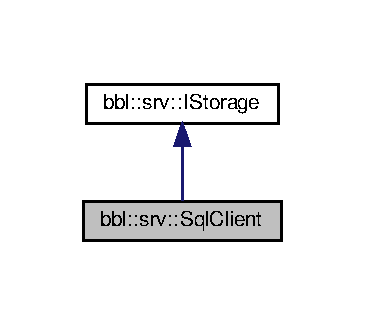
\includegraphics[width=175pt]{classbbl_1_1srv_1_1_sql_client__inherit__graph}
\end{center}
\end{figure}


Collaboration diagram for bbl\+:\+:srv\+:\+:Sql\+Client\+:
\nopagebreak
\begin{figure}[H]
\begin{center}
\leavevmode
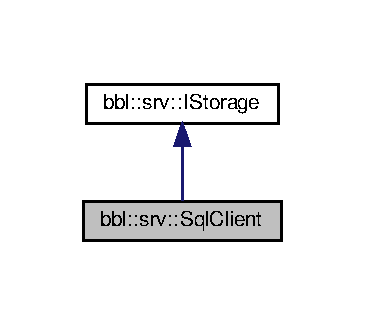
\includegraphics[width=175pt]{classbbl_1_1srv_1_1_sql_client__coll__graph}
\end{center}
\end{figure}
\subsection*{Public Member Functions}
\begin{DoxyCompactItemize}
\item 
\mbox{\Hypertarget{classbbl_1_1srv_1_1_sql_client_a5e36d3c286d32aa8ddf172e1563ead62}\label{classbbl_1_1srv_1_1_sql_client_a5e36d3c286d32aa8ddf172e1563ead62}} 
{\bfseries Sql\+Client} (const std\+::string \&database)
\item 
\mbox{\Hypertarget{classbbl_1_1srv_1_1_sql_client_a9644bdc97fde0a7aeb075f67d789a6f9}\label{classbbl_1_1srv_1_1_sql_client_a9644bdc97fde0a7aeb075f67d789a6f9}} 
{\bfseries Sql\+Client} (const \hyperlink{classbbl_1_1srv_1_1_sql_client}{Sql\+Client} \&)=delete
\item 
\mbox{\Hypertarget{classbbl_1_1srv_1_1_sql_client_a09faaad41f17bd1021c457379307bcd3}\label{classbbl_1_1srv_1_1_sql_client_a09faaad41f17bd1021c457379307bcd3}} 
\hyperlink{classbbl_1_1srv_1_1_sql_client}{Sql\+Client} \& {\bfseries operator=} (const \hyperlink{classbbl_1_1srv_1_1_sql_client}{Sql\+Client} \&)=delete
\item 
\mbox{\Hypertarget{classbbl_1_1srv_1_1_sql_client_ad335279e409901ac94d2dfaf3855a04d}\label{classbbl_1_1srv_1_1_sql_client_ad335279e409901ac94d2dfaf3855a04d}} 
void {\bfseries register\+User} (const std\+::string \&username, const std\+::string \&password) const
\item 
\mbox{\Hypertarget{classbbl_1_1srv_1_1_sql_client_a7f0661b2848724af3b2dc79aca3a8d9f}\label{classbbl_1_1srv_1_1_sql_client_a7f0661b2848724af3b2dc79aca3a8d9f}} 
void {\bfseries login\+User} (const std\+::string \&username, const std\+::string \&password) const
\item 
\mbox{\Hypertarget{classbbl_1_1srv_1_1_sql_client_ade6054df37f4bc4753f029c999e44778}\label{classbbl_1_1srv_1_1_sql_client_ade6054df37f4bc4753f029c999e44778}} 
std\+::vector$<$ std\+::string $>$ {\bfseries get\+Contacts} (const std\+::string \&username) const
\item 
\mbox{\Hypertarget{classbbl_1_1srv_1_1_sql_client_af9522692004b248db03e2b27b2549889}\label{classbbl_1_1srv_1_1_sql_client_af9522692004b248db03e2b27b2549889}} 
std\+::vector$<$ std\+::string $>$ {\bfseries get\+Requests} (const std\+::string \&username) const
\item 
\mbox{\Hypertarget{classbbl_1_1srv_1_1_sql_client_ae9e4dde1aeec2412b7ee1c692f5cb11d}\label{classbbl_1_1srv_1_1_sql_client_ae9e4dde1aeec2412b7ee1c692f5cb11d}} 
void {\bfseries add\+Request} (const std\+::string \&owner, const std\+::string \&contact) const
\item 
\mbox{\Hypertarget{classbbl_1_1srv_1_1_sql_client_abab7af1c3fe96c98c8c4d5b1c3a1389c}\label{classbbl_1_1srv_1_1_sql_client_abab7af1c3fe96c98c8c4d5b1c3a1389c}} 
void {\bfseries accept\+Request} (const std\+::string \&owner, const std\+::string \&contact) const
\item 
\mbox{\Hypertarget{classbbl_1_1srv_1_1_sql_client_adbf1c95f96b24d2cc25d29672d53611d}\label{classbbl_1_1srv_1_1_sql_client_adbf1c95f96b24d2cc25d29672d53611d}} 
void {\bfseries set\+Udp\+Parameters} (const std\+::string \&owner, const std\+::string \&ipv4, const std\+::string \&port) const
\item 
\mbox{\Hypertarget{classbbl_1_1srv_1_1_sql_client_a8055ff59a2b1b019f1d301849bfe11c9}\label{classbbl_1_1srv_1_1_sql_client_a8055ff59a2b1b019f1d301849bfe11c9}} 
std\+::array$<$ std\+::string, 2 $>$ {\bfseries get\+Udp\+Parameters} (const std\+::string \&owner, const std\+::string \&me) const
\end{DoxyCompactItemize}


The documentation for this class was generated from the following files\+:\begin{DoxyCompactItemize}
\item 
Server/include/\+Storage/Sql\+Client.\+hpp\item 
Server/src/\+Storage/Sql\+Client.\+cpp\end{DoxyCompactItemize}

\hypertarget{classbbl_1_1srv_1_1_user}{}\section{bbl\+:\+:srv\+:\+:User Class Reference}
\label{classbbl_1_1srv_1_1_user}\index{bbl\+::srv\+::\+User@{bbl\+::srv\+::\+User}}
\subsection*{Public Member Functions}
\begin{DoxyCompactItemize}
\item 
\mbox{\Hypertarget{classbbl_1_1srv_1_1_user_a3cd17454b095a77a93d8690ab23f0cec}\label{classbbl_1_1srv_1_1_user_a3cd17454b095a77a93d8690ab23f0cec}} 
{\bfseries User} (\hyperlink{classbbl_1_1srv_1_1_i_network_client}{I\+Network\+Client} $\ast$client)
\item 
\mbox{\Hypertarget{classbbl_1_1srv_1_1_user_a2b40e9a0073dc74113a8d9bce7f374f7}\label{classbbl_1_1srv_1_1_user_a2b40e9a0073dc74113a8d9bce7f374f7}} 
{\bfseries User} (const \hyperlink{classbbl_1_1srv_1_1_user}{User} \&)=delete
\item 
\mbox{\Hypertarget{classbbl_1_1srv_1_1_user_a0ca22704d3257634862b7a3b1ebe3a32}\label{classbbl_1_1srv_1_1_user_a0ca22704d3257634862b7a3b1ebe3a32}} 
\hyperlink{classbbl_1_1srv_1_1_user}{User} \& {\bfseries operator=} (const \hyperlink{classbbl_1_1srv_1_1_user}{User} \&)=delete
\item 
\mbox{\Hypertarget{classbbl_1_1srv_1_1_user_a58d16c117e5c0577c793364496e78e20}\label{classbbl_1_1srv_1_1_user_a58d16c117e5c0577c793364496e78e20}} 
bool {\bfseries is\+Logged} () const
\item 
\mbox{\Hypertarget{classbbl_1_1srv_1_1_user_a65d32b6a769c1f7493a5cdf8336e8c87}\label{classbbl_1_1srv_1_1_user_a65d32b6a769c1f7493a5cdf8336e8c87}} 
void {\bfseries signin} (const std\+::string \&username)
\item 
\mbox{\Hypertarget{classbbl_1_1srv_1_1_user_aad7ac7230675f32b0e6591ee704eb222}\label{classbbl_1_1srv_1_1_user_aad7ac7230675f32b0e6591ee704eb222}} 
void {\bfseries signout} ()
\item 
\mbox{\Hypertarget{classbbl_1_1srv_1_1_user_acfe468fe594824191a57d1497f3fa439}\label{classbbl_1_1srv_1_1_user_acfe468fe594824191a57d1497f3fa439}} 
\hyperlink{classbbl_1_1srv_1_1_i_network_client}{I\+Network\+Client} $\ast$ {\bfseries get\+Network\+Part} () const
\item 
\mbox{\Hypertarget{classbbl_1_1srv_1_1_user_a7079d6aefd9d1b930d837039c1b3e7df}\label{classbbl_1_1srv_1_1_user_a7079d6aefd9d1b930d837039c1b3e7df}} 
std\+::string {\bfseries get\+Username} () const
\end{DoxyCompactItemize}


The documentation for this class was generated from the following files\+:\begin{DoxyCompactItemize}
\item 
Server/include/\+Core/User.\+hpp\item 
Server/src/\+Core/User.\+cpp\end{DoxyCompactItemize}

%--- End generated contents ---

% Index
\backmatter
\newpage
\phantomsection
\clearemptydoublepage
\addcontentsline{toc}{chapter}{Index}
\printindex

\end{document}
